% ============================================================
% 整合导言区：国赛格式 + 算法/假设环境 + Draft 提速开关
% 编译方式: latexmk -xelatex (由 VS Code 配置一键调用)
% ============================================================

% ---------- 草稿模式开关 ----------
% 取消下一行注释进入极速草稿模式：图片变方框、关闭超链接书签，
% 编译速度通常提升 3-8 倍，适合改文字/调公式阶段。
\def\FASTDRAFT{}

\ifdefined\FASTDRAFT
  \documentclass[draft,12pt,a4paper]{ctexart}
\else
  \documentclass[fontset=windows,12pt,a4paper]{ctexart}
\fi

% ---------- 页面几何 ----------
\usepackage{geometry}
\geometry{
    paperwidth=210mm, paperheight=297mm,
    left=2.5cm, right=2.5cm,
    top=2.5cm, bottom=2.5cm
}

% ---------- 数学 ----------
\usepackage{amsmath,amsfonts,amssymb,bm,amsthm}

% ---------- 图片与颜色 ----------
\ifdefined\FASTDRAFT
  \usepackage[draft]{graphicx}
\else
  \usepackage{graphicx}
  \DeclareGraphicsExtensions{.pdf,.png,.jpg,.jpeg}
\fi
\usepackage{xcolor}

% ---------- 子图 ----------
\usepackage{subcaption}

% ---------- 表格（三线表 + 复杂表格） ----------
\usepackage{booktabs,tabularx,multirow,array,longtable,colortbl}
\renewcommand{\heavyrulewidth}{2.25pt}
\renewcommand{\lightrulewidth}{0.75pt}
\renewcommand{\cmidrulewidth}{0.75pt}
\renewcommand{\arraystretch}{1.25}

% ---------- 浮动体 ----------
\usepackage{float}

% ---------- 列表 ----------
\usepackage[shortlabels]{enumitem}
\setlist{nosep,leftmargin=1.5em}

% ---------- 算法与代码 ----------
\usepackage{algorithm}
\usepackage{algpseudocode}
\floatname{algorithm}{算法}
\renewcommand{\algorithmicrequire}{\textbf{输入：}}
\renewcommand{\algorithmicensure}{\textbf{输出：}}

\usepackage{listings}
\lstset{
    language=Python,
    basicstyle=\small\ttfamily,
    keywordstyle=\color{blue}\bfseries,
    commentstyle=\color{green!50!black}\itshape,
    stringstyle=\color{orange},
    numbers=left,
    numberstyle=\tiny\color{gray},
    stepnumber=1,
    numbersep=8pt,
    backgroundcolor=\color{gray!10},
    frame=single,
    frameround=tttt,
    breaklines=true,
    showstringspaces=false,
    tabsize=4,
    captionpos=b,
    xleftmargin=2em,
    xrightmargin=1em,
    aboveskip=1em,
    belowskip=1em
}

% ---------- 页眉页脚 ----------
\usepackage{fancyhdr,lastpage}
\pagestyle{fancy}
\fancyhf{}
\fancyfoot[C]{\thepage}
\renewcommand{\headrulewidth}{0pt}

% ---------- 标题格式（国赛推荐） ----------
\ctexset{
    section = {
        number = \chinese{section}、,
        format = \zihao{3}\heiti\bfseries\centering,
        beforeskip = 1.0ex plus 0.5ex minus 0.2ex,
        afterskip  = 1.0ex plus 0.5ex minus 0.2ex
    },
    subsection = {
        format = \zihao{4}\heiti\bfseries\raggedright,
        beforeskip = 0.8ex plus 0.3ex minus 0.1ex,
        afterskip  = 0.8ex plus 0.3ex minus 0.1ex
    },
    subsubsection = {
        format = \zihao{-4}\heiti\bfseries\raggedright,
        beforeskip = 0.5ex plus 0.2ex minus 0.1ex,
        afterskip  = 0.5ex plus 0.2ex minus 0.1ex
    }
}

% ---------- 图表标题格式 ----------
\usepackage{caption}
\captionsetup[figure]{labelsep=space, font=small}
\captionsetup[table]{labelsep=space, font=small}

% ---------- 行距 ----------
\usepackage{setspace}
\setstretch{1.25}

% ---------- 数学定理环境 ----------
\theoremstyle{definition}
\newtheorem{definition}{定义}[section]
\newtheorem{theorem}{定理}[section]
\newtheorem{lemma}{引理}[section]
\newtheorem{assumption}{假设}[section]

% ---------- 绘图（按需启用） ----------
\usepackage{tikz}
\usetikzlibrary{shapes.geometric, arrows.meta, positioning, calc}
\usepackage{pgfplots}
\pgfplotsset{compat=1.18}

% TikZ 外部化缓存（需 -shell-escape）
\ifdefined\FASTDRAFT
\else
  \usetikzlibrary{external}
  \tikzexternalize[prefix=tikz-cache/]
\fi

% ---------- 超链接（务必靠后） ----------
\ifdefined\FASTDRAFT
  \usepackage[draft,hidelinks,bookmarks=false,unicode=true]{hyperref}
\else
  \usepackage[hidelinks,bookmarks=true,bookmarksnumbered=true,unicode=true]{hyperref}
\fi
\usepackage{cleveref}



% ---------- 自定义命令 ----------
\newcommand{\diff}{\mathrm{d}}
\newcommand{\E}{\mathrm{E}}
\newcommand{\Var}{\mathrm{Var}}
\newcommand{\Cov}{\mathrm{Cov}}
\DeclareMathOperator*{\argmin}{arg\,min}
\DeclareMathOperator*{\argmax}{arg\,max}

% ============================================================
% 正文开始
% ============================================================
\begin{document}

% ---------- 论文骨架所需补充命令（模板导言区未定义） ----------
\newcommand{\keywords}[1]{\par\vspace{6pt}\noindent\textbf{关键词：#1}\par}

\renewcommand{\lstlistingname}{代码}

%================ 首页三要素 =================
\begin{center}
  {\huge\bfseries 基于\textbf{TOA定位模型}的\textbf{火箭残骸音爆定位}\par}
\end{center}


%================ 摘要 =================
%================ 摘要 =================
\begin{center}
  {\zihao{4}\bfseries \textbf{摘\quad 要}}
\end{center}
\vspace{0.1cm}

针对问题一，考虑到音爆信号以恒定声速传播、到达时刻与传播距离成线性关系这一物理约束，建立了\textbf{到达时间（TOA）定位模型}，
将音爆发生时刻与三维位置一并作为未知量，利用\textbf{平方差分线性化}求取初值、\textbf{非线性最小二乘}做迭代精细化，
并辅以\textbf{多初值扫描}排除虚假解。理论分析表明，4个未知量\textbf{至少需要4台}监测设备定解，
但4台恰好定解不具备任何检错能力，\textbf{残差分析、留一交叉验证、蒙特卡洛模拟}显示，针对精确计算音爆位置的现实问题，4台不足以较好的排除系统性误差，实际布置应\textbf{不少于5台}。
对题目给出的7台设备数据，通过\textbf{4台子集枚举}与\textbf{残差检验}判定设备D、F记录异常（残差分别为$-19.4$\,km和$-16.2$\,km），
予以剔除；以A、B、C、E、G五台联合解算，得到残骸音爆位置为\textbf{东经110.499$^\circ$、北纬27.311$^\circ$、高程约855\,m}，
音爆时刻为系统时钟后\textbf{19.3\,s}。

针对问题二，将单残骸TOA模型扩展为\textbf{多残骸联合定位模型}，引入\textbf{0-1关联变量}刻画设备读数与残骸的对应关系，
建立\textbf{混合整数非线性优化(MINLP)}目标；采用\textbf{4站初步筛选+全站联合验真}的两层策略，
将搜索空间从$(n!)^m$压缩到$n^m$次解析求解，再用全部设备的TOA残差筛选真解、以\textbf{精确覆盖}保证一对一关联。
理论分析表明，4个残骸需至少\textbf{4台}设备方可定解，但4台无冗余校验能力，工程上应布置\textbf{不少于5台}；
\textbf{位置精度因子（PDOP）}计算验证了5台配置时精度显著提高。

针对问题三，利用问题二模型对题目给出的7台设备、28个到达时刻数据进行求解。枚举$4^7=16384$种单事件组合后，
经\textbf{物理边界过滤}、\textbf{利用全站残差精细化}，仅保留4个候选，再由\textbf{精确覆盖}唯一确定4个残骸的时空状态。
解得4个残骸的音爆时刻分别为\textbf{11.9999\,s}、\textbf{13.0014\,s}、\textbf{14.0000\,s}、\textbf{15.0000\,s}，
位置呈十字对称分布；全部28个残差落在\textbf{$\pm0.6$\,ms}以内，7台设备全部可靠。求解过程中未使用5秒时间窗约束，
但输出结果自然满足该条件，说明模型鉴别力来自\textbf{全站联合一致性}而非时间窗约束。

针对问题四，在$\pm0.5$\,s随机计时误差下对关联--定位模型做三项修正：验真阈值按噪声的\textbf{蒙特卡洛传播规律}统计标定（严格阈值取RMSE$<0.55$\,s且max$|$残差$|<0.65$\,s）、\textbf{多组低条件数4台组合}批量解析抗组合退化、\textbf{分级阈值加剩余读数补全}的容错机制，修正后\textbf{关联成功率回到100\%}。对问题三数据叠加随机误差做300次蒙特卡洛实验：7台现状3D误差95\%分位达\textbf{1224\,m}、\textbf{10.4\%}的实验超过1\,km，瓶颈在高程方向。据此按PDOP精度预算设计加密监测设备网：原7台不动，新增中心1台、内环4台（15\,km）、外环8台（45\,km）共\textbf{20台}，配合7台确定关联、20台提升精度的两阶段求解策略，用问题三定位结果正向模拟新监测设备网数据并盲解反演，3D误差95\%分位降至\textbf{457\,m}、最大\textbf{810\,m}，超标比例\textbf{0\%}，满足误差小于1\,km的要求。六项稳健性压力测试进一步表明，模型的关联鉴别力在各类极端噪声形态下、\textbf{均保持稳健}，能力边界为单站2\,s级粗差与超出设计值60\%以上的噪声水平。

\vspace{6pt}
\keywords{火箭残骸音爆定位; TOA定位模型; 多残骸联合定位;  精确覆盖}
\newpage

%================ 1 问题重述 =================
\section{问题重述}
\subsection{问题背景}
多级火箭部件分离坠落，过程中残骸跨音速飞行并产生音爆。为实现残骸的快速回收，只需要推算残骸发生音爆时的空中位置，
进便可通过弹道外推实现落点的快速精准定位。本题即要求我们通过理论落区内布置的多台震动波监测设备，
根据音爆抵达各台设备的时间和各设备位置推算出音爆发生的位置。

设音爆发生点为$S=(x,y,z)$，发生时刻为$\tau_0$，监测设备$i$的坐标为$P_i=(x_i,y_i,z_i)$，记录到的音爆抵达时刻为$t_i$，音爆在空气中的传播速度为$c$，则有
\begin{equation}
  \big\|S-P_i\big\|=c\,(t_i-\tau_0),\qquad i=1,2,\dots,n,
  \label{eq:background-toa}
\end{equation}
式\eqref{eq:background-toa}描述了音爆点位置、发生时刻与各台设备观测时刻之间的几何约束，是全文各问建模的、\textbf{共同出发点}。题目给定$c=340$\,m/s，计算两点间距离时可忽略地面曲率，纬度每度距离近似为111.263\,km，经度每度距离近似为97.304\,km。

\subsection{问题的提出}
基于上述背景，我们需解决以下问题：
\begin{enumerate}[label=\arabic*.]
  \item \textbf{问题一（单残骸定位）}：分析精准确定空中单个残骸音爆位置（经度、纬度、高程）和时间至少需要布置几台监测设备；并从题目给出的7台设备观测数据（三维坐标与音爆抵达时间）中选取合适的数据，计算残骸发生音爆时的位置和时间。
  \item \textbf{问题二（多残骸归属判定）}：空中有4个残骸时，每台设备按时间先后收到4组震动波。建立数学模型，判定设备接收到的各组震动波来自哪一个残骸，并分析确定4个残骸的音爆位置和时间至少需要布置多少台监测设备。
  \item \textbf{问题三（多残骸解算）}：利用问题二的模型，从题目给出的7台设备、每台4组抵达时间的数据中选取合适的数据，确定4个残骸发生音爆时的位置和时间（各残骸音爆时刻互不相同，但差别不超过5\,s）。
  \item \textbf{问题四（含误差修正与布站设计）}：设备记录时间存在0.5\,s随机误差，修正问题二的模型；通过对问题三数据叠加随机误差给出算例并分析结果误差；若时间误差无法降低，给出一种实现精准定位（误差$<1$\,km）的方案，并模拟所需设备位置与观测数据加以验证。
\end{enumerate}

%================ 2 问题分析 =================
\section{问题分析}

我们的总体思路如下：先将各台设备的经纬高坐标换算到局部直角坐标系，对观测数据做初步检查；随后以式\eqref{eq:background-toa}为核心建立定位模型，问题一解决单残骸定位与数据筛选，问题二、三在其上扩展出归属判定机制，问题四再针对时间误差做模型修正与布站设计，四个问题层层递进。

\begin{enumerate}[label=\arabic*.]
  \item \textbf{问题一}：该问题属于\textbf{几何定位问题}。每台设备提供1个观测方程，而未知量有位置3个坐标与音爆时刻共4个，故方程数与未知量数的平衡关系决定了设备数量的下限。难点有三：其一，观测方程关于未知量是非线性的，需设计可靠的初值与迭代策略，避免收敛到高程为负之类的虚假解；其二，7台设备中可能混有异常记录，直接用全部数据解算会污染结果，需借助冗余观测做检验；其三，题目要求"选取合适的数据"，意味着数据筛选本身就是求解的一部分。拟建立TOA定位模型，用线性化方法提供初值、非线性最小二乘精细化，并以子集枚举和残差检验完成异常数据的识别与剔除。
  \item \textbf{问题二}：该问题属于\textbf{组合关联与定位问题}。4个残骸产生4组音爆，每台设备按时间先后记录4个到达时刻，但设备不知道第$k$个读数来自哪个残骸。难点在于关联未知使观测方程数与未知量数的平衡关系变得复杂，且组合爆炸（$4^7=16384$种单事件候选）要求高效的剪枝与验真机制。拟建立多残骸TOA联合模型，4站初步筛选、利用全站残差验真筛选候选、精确覆盖保证一对一关联，并分析最少设备数。
  \item \textbf{问题三}：该问题属于\textbf{多残骸定位的实例验证问题}。在问题二模型的框架下，代入7台设备各4组抵达时刻的具体数据，求解4个残骸的时空状态，并验证数据质量与5秒时间窗约束。拟沿用问题二的4站初步筛选+全站验真策略，输出各残骸位置、时刻及设备关联方案，以残差诊断验证结果可靠性。
  \item \textbf{问题四}：该问题属于\textbf{误差环境下的模型修正与监测设备网设计问题}。计时误差$\pm0.5$\,s使正确关联的残差从接近零抬升到噪声本身的量级，问题二的严格阈值与单个4台组合在误差环境下会系统性误杀真解，需按噪声统计规律重新标定鉴别阈值并增设容错兜底；误差分析需用蒙特卡洛模拟把计时误差传播到定位域，量化精度是否达标；若误差不达标且无法降低，则需通过加密监测设备网改善观测几何，以位置精度因子（PDOP）做精度预算确定台数与布局，并用问题三的定位结果正向模拟台站数据、反演验证。拟保留``枚举—验真—覆盖''框架骨架，修正其阈值标定、初始4台组合生成与容错机制，再以7 台确定关联、20 台提升精度的两阶段策略适配加密监测设备网。
\end{enumerate}

%================ 3 模型假设 =================
\newpage
\section{模型假设}

\textbf{1. 声速恒定、忽略地面曲率：}音爆以恒定声速$c=340$\,m/s沿直线传播，不考虑风速、温度分层等因素对声速的影响；忽略地面曲率，忽略声速局地起伏折算后的距离偏差。

\textbf{2. 计时与观测：}各台设备时钟严格同步，记录的音爆抵达时刻相对于同一系统时钟零时；问题一至问题三中观测时刻的误差仅为数值舍入量级；问题四中各读数含$\pm0.5s$的独立均匀分布随机计时误差。

\textbf{3. 音爆事件：}音爆可视为发生在空中某一点的瞬时点声源事件，各台设备接收到的信号均由该点发出；不同残骸的音爆事件相互独立，发生时刻互不相同且差别不超过$5$\,s。


\textbf{4. 信号可分辨：}同一设备接收到的不同残骸音爆信号在时域上互不重叠，设备能够按时间先后无歧义地输出各组到达时刻读数。

\textbf{5. 误差统计稳定：}问题四中设备计时误差的概率分布（均匀分布、零均值、各读数相互独立）在整个观测时段内保持不变，其统计规律可通过有限次蒙特卡洛实验标定验真阈值。
%================ 4 符号说明 =================
\section{符号说明}
我们主要用到以下符号。
\begin{table}[H]\centering
  \caption{主要符号说明}\label{tab:symbol}
  \small
  \begin{tabular}{ccc}
    \toprule
    \textbf{符号} & \textbf{说明} & \textbf{单位} \\
    \midrule
    $S=(x,y,z)$ & 音爆发生点在局部坐标系中的坐标 & m \\
    $P_i=(x_i,y_i,z_i)$ & 第$i$台监测设备在局部坐标系中的坐标 & m \\
    $t_i$ & 第$i$台设备记录的音爆抵达时刻 & s \\
    $\tau$ & 音爆发生时刻 & s \\
    $c$ & 音爆传播速度，取340 & m/s \\
    $r_i$ & 第$i$台设备的定位残差 & m \\
    $K_{\mathrm{lon}},K_{\mathrm{lat}}$ & 经度、纬度每度折合距离 & m/° \\
    $n$ & 参与解算的设备台数 & --- \\
    \bottomrule
  \end{tabular}
\end{table}

%================ 5 数据预处理与结构特征 =================
\newpage
\section{数据预处理与结构特征}
\subsection{数据来源与规模}
问题一使用的数据为题目给出的7台监测设备（编号A至G）的三维坐标与音爆抵达时刻，共7组记录，每组含经度、纬度、高程、抵达时刻4个字段，如表\ref{tab:q1-data}所示。

\begin{table}[H]\centering
  \caption{问题一监测设备坐标与音爆抵达时刻}\label{tab:q1-data}
  \small
  \begin{tabular}{ccccc}
    \toprule
    \textbf{设备} & \textbf{经度(°)} & \textbf{纬度(°)} & \textbf{高程(m)} & \textbf{音爆抵达时间(s)} \\
    \midrule
    A & 110.241 & 27.204 & 824 & 100.767 \\
    B & 110.780 & 27.456 & 727 & 112.220 \\
    C & 110.712 & 27.785 & 742 & 188.020 \\
    D & 110.251 & 27.825 & 850 & 258.985 \\
    E & 110.524 & 27.617 & 786 & 118.443 \\
    F & 110.467 & 27.921 & 678 & 266.871 \\
    G & 110.047 & 27.121 & 575 & 163.024 \\
    \bottomrule
  \end{tabular}
\end{table}


\subsection{数据可视化与结构特征}
7台设备大体散布在$0.9°\times0.8°$的经纬范围内，台间距数十公里，对落区中部形成包围态势，几何布局有利于三维定位。

对抵达时刻做初步检查：最早与最晚记录相差约166\,s，若全部来自同一音爆点，对应传播距离相差约56\,km，而监测设备网尺度与此量级相当，单从时刻大小无法排除任何一台设备。因此，数据是否全部有效不能靠先验判断，必须放到定位模型中检验——这正是问题一要求"选取合适的数据"的原因，相关检验与结果在第六部分给出。


%================ 6 问题一 =================
\newpage
\section{问题一：单个残骸的音爆定位}

对单个残骸，音爆发生点$S=(x,y,z)$与发生时刻$\tau_0$均为未知量，连同式\eqref{eq:background-toa}即构成定位模型。采用到达时间（TOA）定位方法。

图\ref{fig:toa-principle}给出了TOA定位的球面交汇几何示意：每台设备确定一个以自身为球心、声波传播距离为半径的球面，音爆点即位于这些球面的交汇区域。未知量共4个（3维坐标加音爆时刻），每台设备提供1个球面约束，故理论上至少需要4个球面方可唯一确定交点。

\begin{figure}[H]
  \centering
  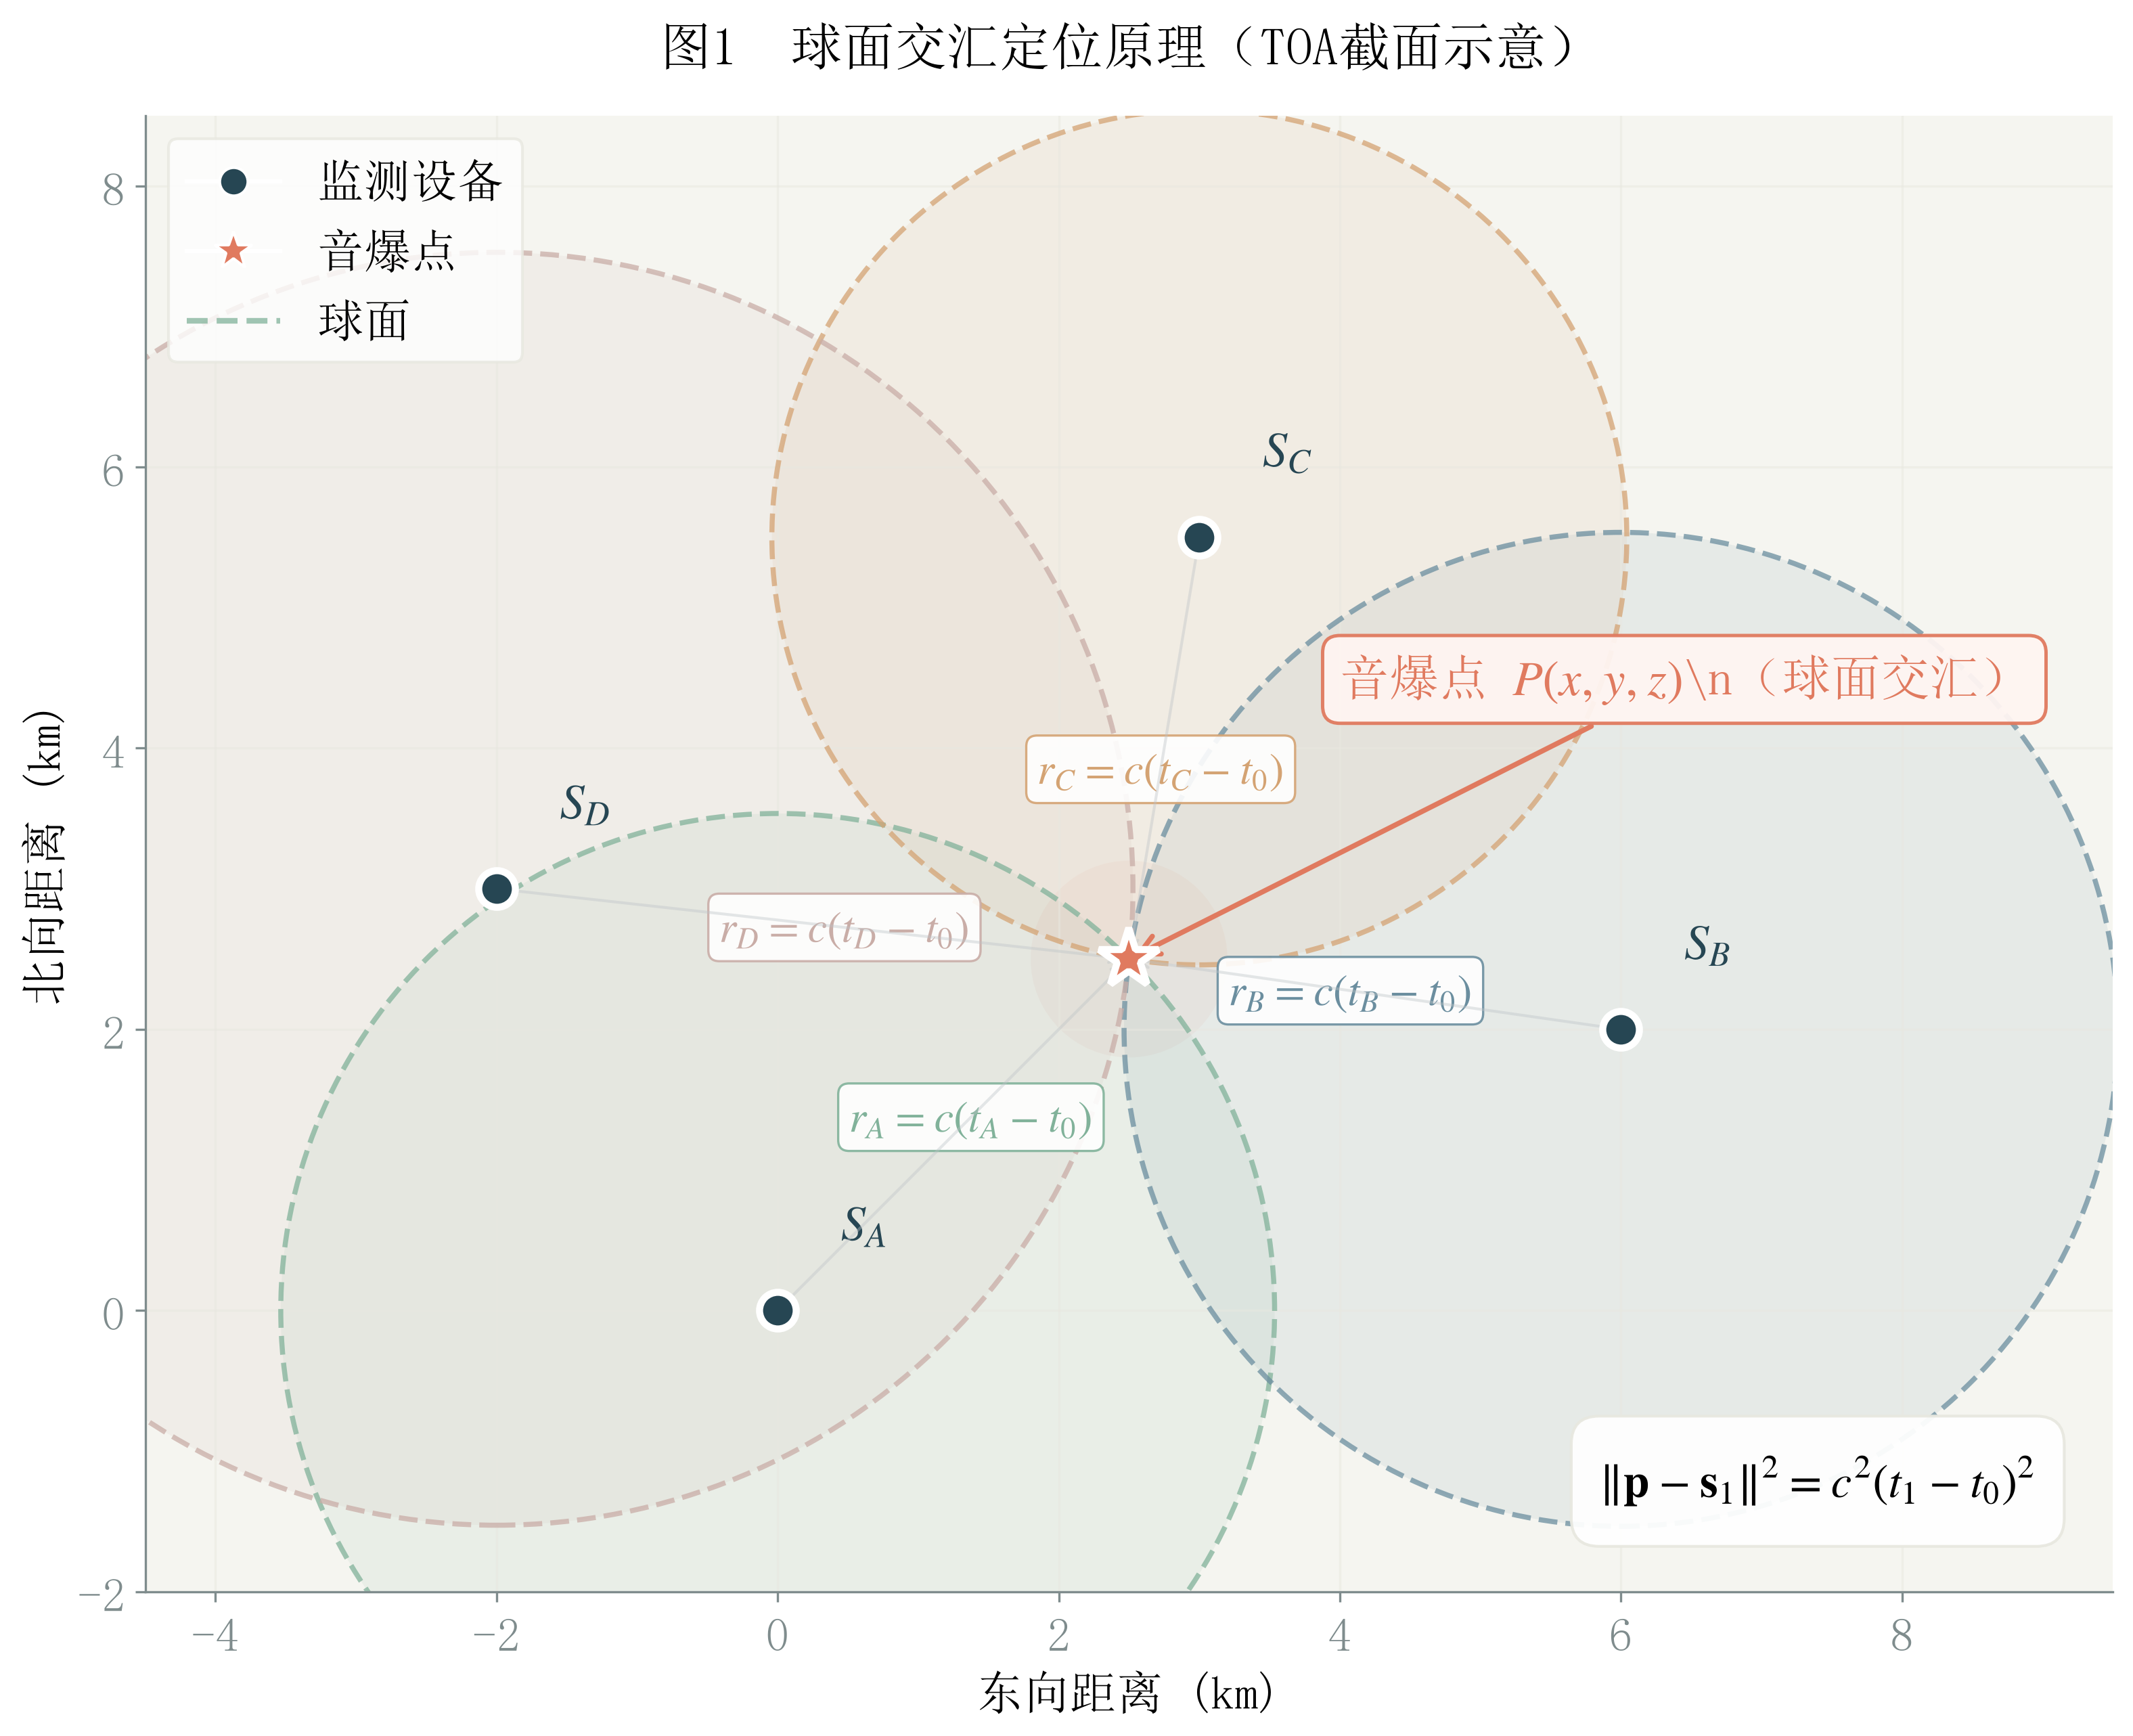
\includegraphics[width=0.9\textwidth]{output/figs/球面交汇定位原理.png}
  \caption{球面交汇定位原理示意}\label{fig:toa-principle}
\end{figure}

式\eqref{eq:background-toa}的几何含义是：音爆点位于以设备$i$为球心、$c(t_i-\tau_0)$为半径的球面上，若干球面的交点即为所求。未知量共4个，每台设备提供1个方程，故\textbf{理论最少需要4台设备}。但4台时方程数与未知量数恰好相等，方程组被唯一确定，任何错误数据都会被原样吸收进解中，且球面交点可能出现高程为负的镜像虚假解，没有任何冗余可用于检错。因此实际布置应\textbf{不少于5台}，用冗余观测换取检错与平差能力。题目给出7台数据，因此我们还需要判断数据是否全部可用。

将式\eqref{eq:background-toa}两边平方并展开，得
\begin{equation}
  \|S\|^2-2P_i\cdot S+\|P_i\|^2=c^2t_i^2-2c^2t_i \tau_0+c^2\tau_0^2.
  \label{eq:squared}
\end{equation}
用第$i$式减去第1式，二次项$\|S\|^2$与$c^2\tau_0^2$被消去，得到关于$(x,y,z,\tau_0)$的线性方程组
\begin{equation}
  2(P_i-P_1)\cdot S-2c^2(t_i-t_1)\,\tau_0=\|P_i\|^2-\|P_1\|^2-c^2\big(t_i^2-t_1^2\big),
  \qquad i=2,\dots,n,
  \label{eq:linear}
\end{equation}
对其做最小二乘解即得定位粗值。需要说明的是，平方操作松弛了原方程的约束（平方后$t_i-\tau_0$的符号信息丢失），粗值可能偏离真解甚至落到错误分支，只能作为迭代起点。

定义残差
\begin{equation}
  r_i(S,\tau_0)=\underbrace{\|S-P_i\|}_{\text{geometric distance}}-\underbrace{c\,(t_i-\tau_0)}_{\text{sonic distance}},\qquad i=1,\dots,n,
  \label{eq:residual}
\end{equation}
其物理含义为：当前解下点$S$到设备$i$的直线距离与声波在$t_i-\tau_0$内传播距离之差，单位是米。若解正确且数据无误，所有$r_i=0$；$|r_i|$越大，说明第$i$台设备的观测与该解越矛盾。以粗值为初值，用scipy默认的Trust Region Reflective算法求解
\begin{equation}
  (S^{*},\tau_0^{*})=\argmin_{S,\,\tau_0}\ \sum_{i=1}^{n} r_i^2(S,\tau_0).
  \label{eq:lsq}
\end{equation}
该可能问题存在多个局部极小，我们从收敛结果中选取残差最小且物理合理（高程为正、$\tau_0$落在观测时间窗附近）的解。完整流程如算法\ref{alg:q1}所示。

\begin{algorithm}[H]
\caption{问题一求解流程}\label{alg:q1}
\begin{algorithmic}[1]
\Require 设备坐标$P_i$与抵达时刻$t_i$（$i=1,\dots,7$），声速$c$
\Ensure 音爆位置$S^{*}$、时刻$\tau_0^{*}$及参与解算的设备集合
\State 将经纬高换算为局部直角坐标
\State 遍历全部$\binom{7}{4}=35$个4台组合：由式\eqref{eq:linear}求初值，多初值非线性精细化式\eqref{eq:lsq}，记录各组合的解与RMS残差
\State 对比各组合残差量级，筛查异常设备
\State 以筛查后的5台设备联立解算，按式\eqref{eq:residual}计算全部7台设备的残差，确认异常并剔除
\State 对保留设备做4台留一交叉验证与回测残差对比，检验解的稳健性
\State \Return 五台联合解$(S^{*},\tau_0^{*})$
\end{algorithmic}
\end{algorithm}

对35个4台组合逐一求解，结果呈现清晰的二分规律：凡包含设备D或F的组合，RMS残差均在1.5\,km至6.5\,km之间，其中个别``零残差''组合的解落在高程$-5.5$万\,m至$-25.8$万\,m的荒谬位置，属虚假解，直接排除；而只从$\{\mathrm{A,B,C,E,G}\}$中取台的组合，残差均在几十至几百米，且解落在合理空域。这提示D、F的记录与其余设备不属于同一事件。

以A、B、C、E、G五台联合解为基准，按式\eqref{eq:residual}计算全部7台设备的残差，结果如表\ref{tab:residual}所示。D、F的残差分别达$-19.4$\,km和$-16.2$\,km，折合时间矛盾约57\,s和48\,s，远超任何合理的观测误差，最可能的解释是这两台设备记录到的是其他残骸的音爆或记录故障。据此\textbf{判定D、F为异常数据并剔除}，参与最终解算的为A、B、C、E、G五台。

\begin{table}[H]\centering
  \caption{五台联合解下各设备的残差}\label{tab:residual}
  \small
  \begin{tabular}{cccc}
    \toprule
    \textbf{设备} & \textbf{残差(m)} & \textbf{折合时间(s)} & \textbf{判定} \\
    \midrule
    A & $+58$ & $+0.17$ & 有效 \\
    B & $+195$ & $+0.57$ & 有效 \\
    C & $-642$ & $-1.89$ & 有效 \\
    D & $-19371$ & $-56.97$ & \textbf{异常，剔除} \\
    E & $+483$ & $+1.42$ & 有效 \\
    F & $-16174$ & $-47.57$ & \textbf{异常，剔除} \\
    G & $-95$ & $-0.28$ & 有效 \\
    \bottomrule
  \end{tabular}
\end{table}


剔除D、F后，A、B、C、E、G五台联合解为：音爆位置\textbf{东经110.4989°、北纬27.3105°、高程855\,m}，音爆时刻为系统时钟后\textbf{19.313\,s}，RMS残差373\,m。为回答4台是否够用，表\ref{tab:candidates}列出其中两个4台子集的解作对比。

\begin{table}[H]\centering
  \caption{四台子集解与五台联合解对比}\label{tab:candidates}
  \small
  \begin{tabular}{cccccc}
    \toprule
    \textbf{组合} & \textbf{经度(°E)} & \textbf{纬度(°N)} & \textbf{高程(m)} & $\tau_0$\textbf{(s)} & \textbf{RMS残差(m)} \\
    \midrule
    ABCG & 110.5064 & 27.3002 & 1138 & 18.79 & 62 \\
    ABEG & 110.4978 & 27.3143 & 1154 & 19.09 & 53 \\
    ABCEG（5台） & 110.4989 & 27.3105 & 855 & 19.31 & 373 \\
    \bottomrule
  \end{tabular}
\end{table}

两4台子集解的内部RMS分别仅62\,m与53\,m，看似完美拟合了各自数据；但二者水平相距1.78\,km，\textbf{差异显著}。为判断该差异是否源于随机噪声，
对五台数据施加不同水平的随机扰动后重复求解300次，统计解的自然散布，结果如表\ref{tab:monte}所示。

\begin{table}[H]\centering
  \caption{蒙特卡洛噪声散布评估（300次重复，95\%半径）}\label{tab:monte}
  \small
  \begin{tabular}{lcc}
    \toprule
    \textbf{噪声来源} & \textbf{水平散布} & \textbf{高程散布} \\
    \midrule
    坐标量化$\pm0.0005^\circ$ + 时刻舍入$\pm0.0005$\,s & $\approx87$\,m & $\pm10$\,m \\
    $\pm0.5$\,s时间误差（问题四最坏假设） & $\approx300$\,m & $\pm37$\,m \\
    \bottomrule
  \end{tabular}
\end{table}

ABCG与ABEG相距1.78\,km，是噪声级散布的6$\sim$20倍，因此这不是噪声级分歧，而是\textbf{系统性偏差}。具体指向：五台解下C的残差为$-1.89$\,s、E为$+1.42$\,s，方向相反、量级相当——C、E中至少一台存在坐标或钟差系统错误，但现有数据无法判定该剔哪一台（剔C得ABEG，剔E得ABCG，残差几乎同样小）。

我们最终选择\textbf{5台联合解}而非4台，还考虑到了如下因素：（1）4台4方程4未知数恰好定解，残差趋零是数学自动保证，不含任何检错能力。ABCG、ABEG、ACEG三个4台组合残差都只有50$\sim$90\,m，却给出互差1.5$\sim$3.5\,km的三个自洽答案，4台无法鉴别哪一个更准确。
而第5台能提供冗余与裁判能力，有1个冗余自由度，残差更能反映数据质量。
 （2）5台对系统偏差有中和作用：C、E偏差方向相反，5台最小二乘将其折中，解落在两簇候选之间，否则押注任何单一4台组合都可能把1.5\,km系统误差照单全收。



为检验上述结论的稳健性，我们对$\{\mathrm{A,B,C,E,G}\}$进行\textbf{留一交叉验证}，观察其4台子集解的聚散程度，结果如表\ref{tab:vote}所示。其中4解收敛到东经110.499°$\sim$110.506°、北纬27.300°$\sim$27.314°、高程800$\sim$1150\,m这一簇内，五台联合解接近簇中心；仅ACEG一票偏离3.5\,km，且$\tau_0$相差约5\,s，明显离群。多数表决与最小二乘相互印证，说明定位结果是稳健的；离群值同时提示水平方向存在\textbf{系统性不确定度}。

\begin{table}[H]\centering
  \caption{留一交叉验证结果}\label{tab:vote}
  \small
  \begin{tabular}{cccccc}
    \toprule
    \textbf{子集} & \textbf{经度(°E)} & \textbf{纬度(°N)} & \textbf{高程(m)} & $\tau_0$\textbf{(s)} & \textbf{是否入主簇} \\
    \midrule
    ABCE & 110.4986 & 27.3101 & 798 & 19.17 & 是 \\
    ABCG & 110.5064 & 27.3002 & 1138 & 18.79 & 是 \\
    ABEG & 110.4978 & 27.3143 & 1154 & 19.09 & 是 \\
    BCEG & 110.4991 & 27.3108 & 822 & 19.40 & 是 \\
    ACEG & 110.4658 & 27.3332 & 1097 & 24.15 & 否（偏离3.5\,km） \\
    \bottomrule
  \end{tabular}
\end{table}

\begin{figure}[H]
  \centering
  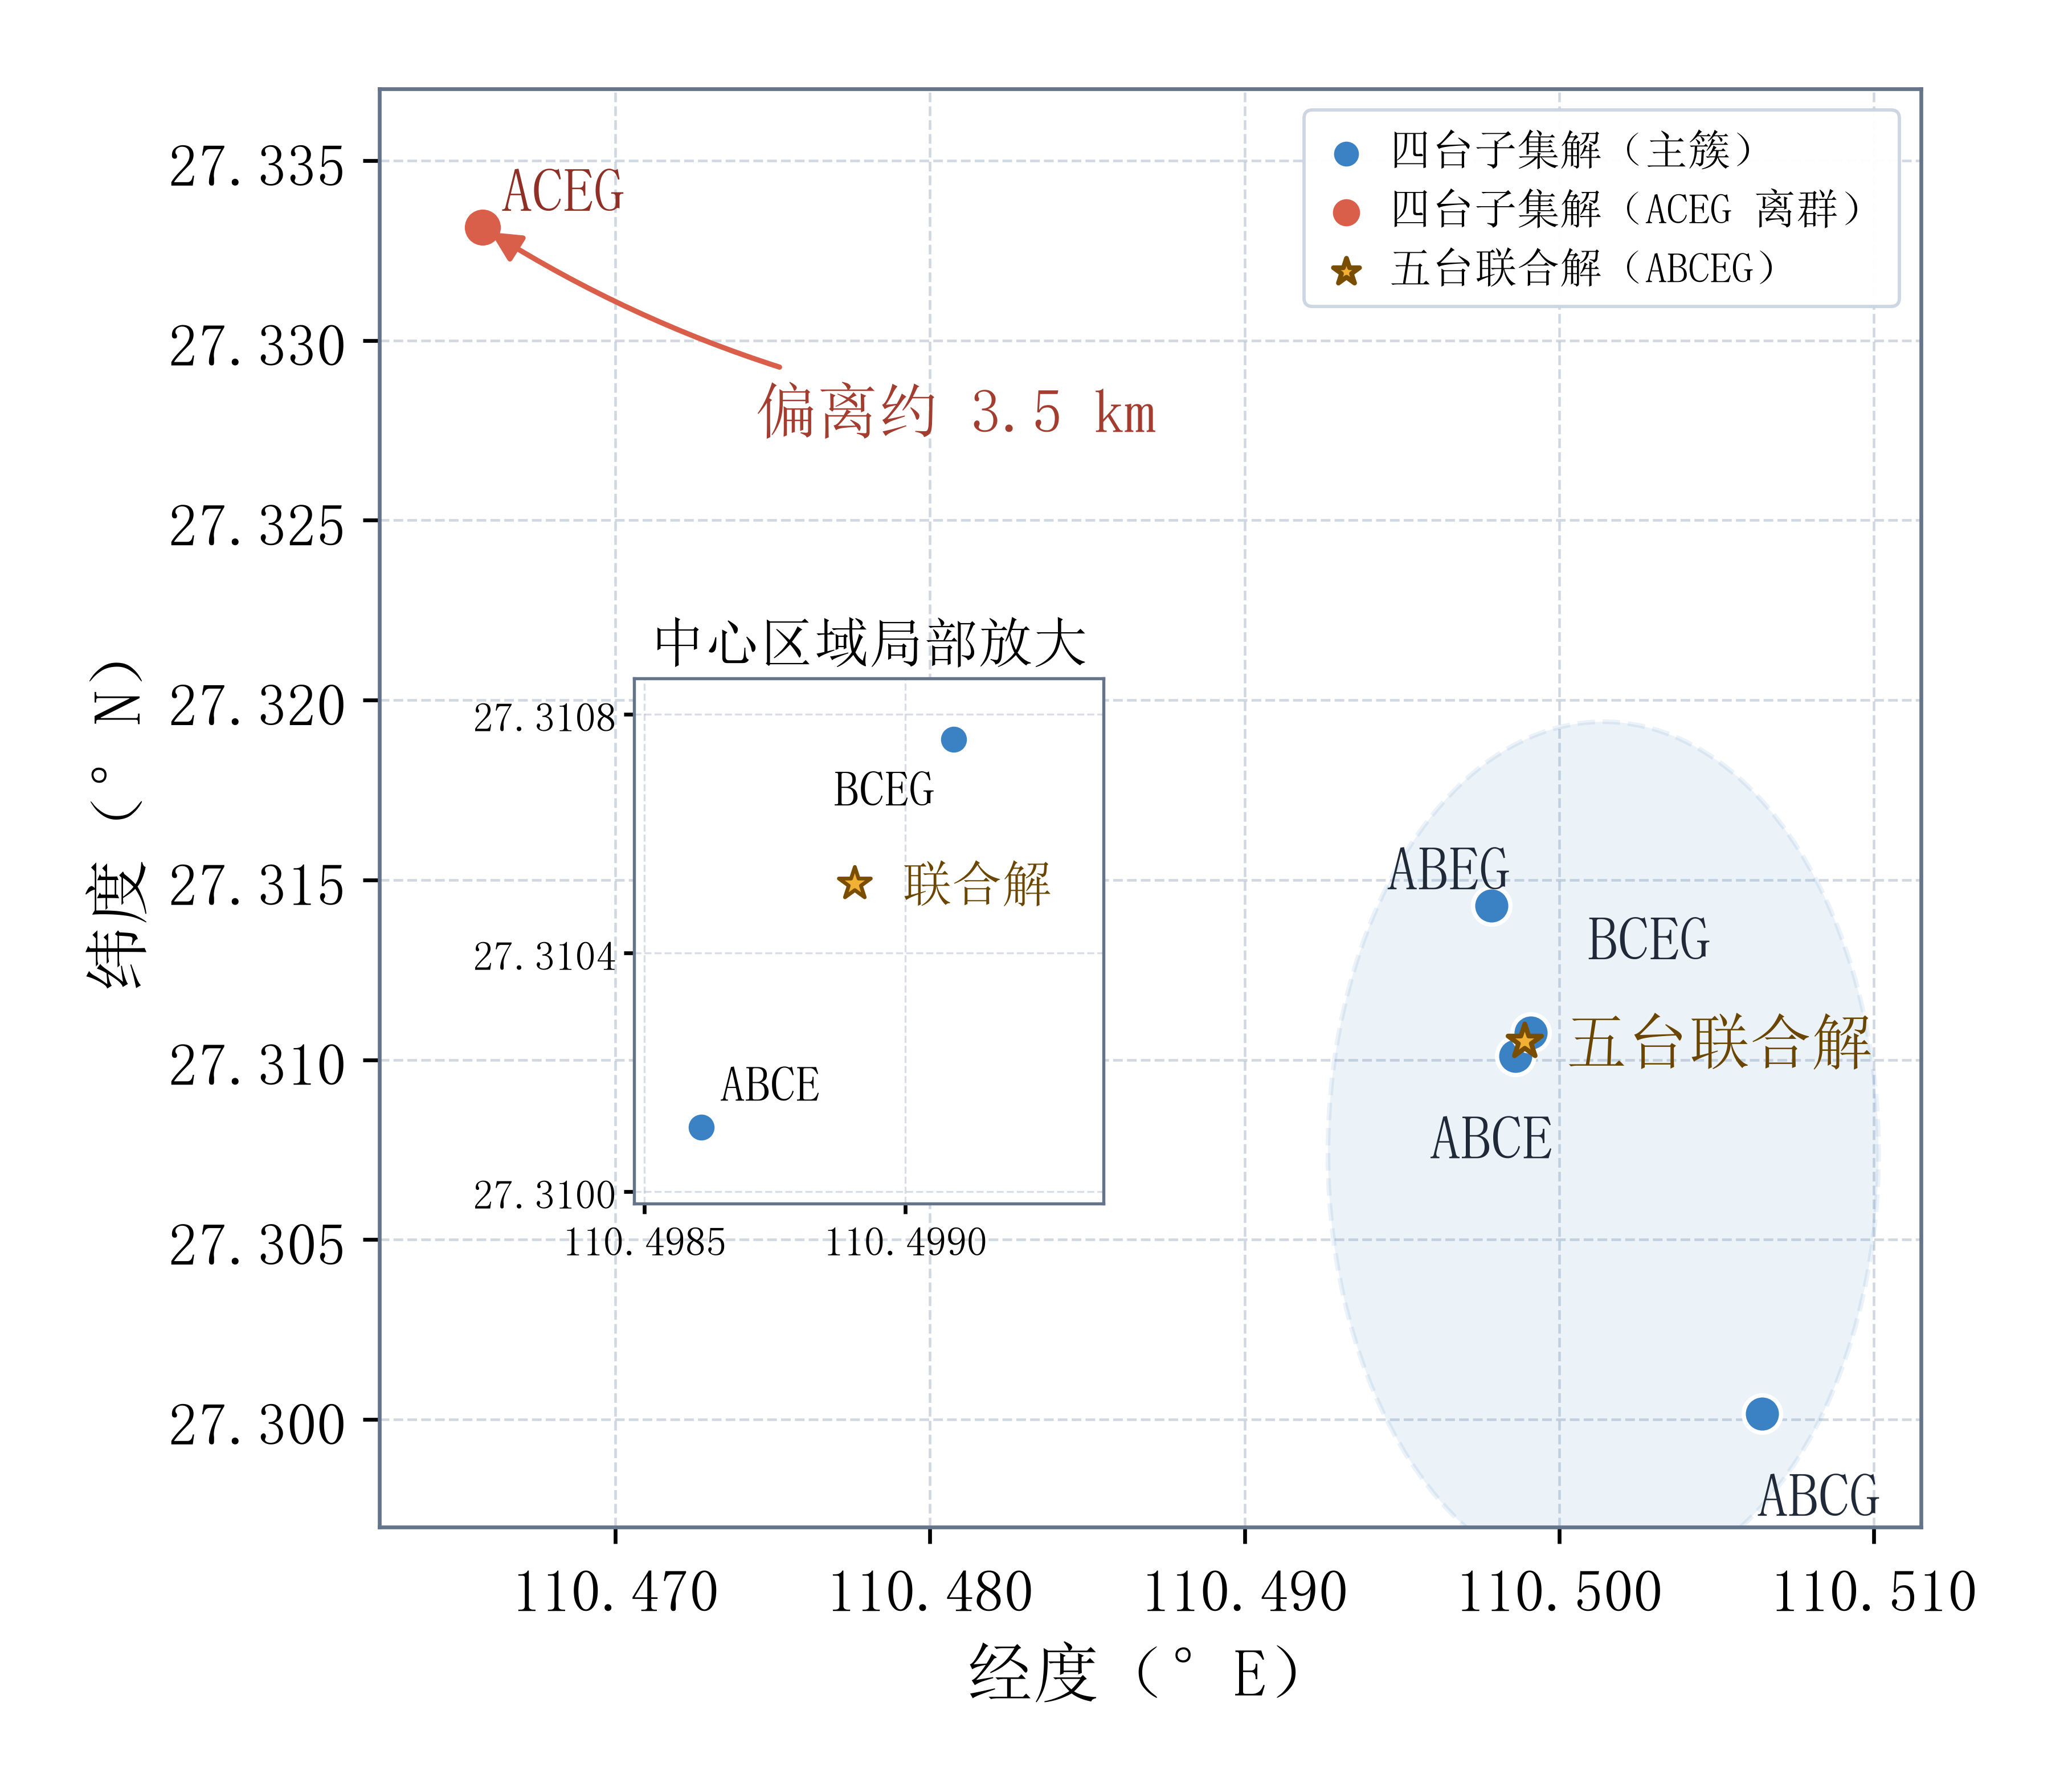
\includegraphics[width=0.72\textwidth]{output/figs/q1_留一交叉验证散点图.png}
  \caption{四台子集解与五台联合解的水平分布}\label{fig:vote}
\end{figure}

以ABCG和ABEG两个4台解分别回测全部7台设备的残差，结果如表\ref{tab:backtest}所示。ABCG解回测设备E的残差高达$+1413$\,m（$+4.16$\,s），ABEG解回测设备C的残差高达$-1067$\,m（$-3.14$\,s），他们互相认为对方核心成员异常；
而五台联合解对C、E的残差分别为$-642$\,m与$+483$\,m，方向相反、量级对称，恰好折中。这说明4台解的内部RMS$\approx$60\,m很可能是维度决定的假象，一旦回测未参与设备，RMS立刻暴涨；。

\begin{table}[H]\centering
  \caption{4台解回测残差对比（单位：m）}\label{tab:backtest}
  \small
  \begin{tabular}{cccc}
    \toprule
    \textbf{设备}  & \textbf{ABCG残差} & \textbf{ABEG残差}& \textbf{五台残差} \\
    \midrule
    A & $+87$  & $+76$ & $+58$ \\
    B & $+3$   & $-0$   & $+195$ \\
    C & $-4$      & $-1067$ & $-642$ \\
    D     & $-18201$   & $-19871$  & $-19371$ \\
    E     & $+1413$ & $+0$   & $+483$ \\
    F      & $-15163$   & $-16671$   & $-16174$ \\
    G  & $-87$  & $-76$ &  $-95$ \\
    \midrule
    \textbf{内部RMS} & \textbf{61.7} & \textbf{53.4} & \textbf{373.0} \\
    \textbf{回测RMS} & \textbf{634.4} &  \textbf{479.7} &  \textbf{373.0} \\
    \bottomrule
  \end{tabular}
\end{table}

综合以上分析，问题一的结论为：精准确定单个残骸的音爆位置与时刻，\textbf{理论最少需4台监测设备，实际应布置不少于5台}以获得检错与平差的能力；
题目7台设备中D、F记录异常予以剔除，由A、B、C、E、G解得音爆位置为\textbf{东经110.499°、北纬27.311°、高程约855\,m}，
音爆时刻为系统时钟后\textbf{19.3\,s}；该结果存在不确定度,主要由个别台站不可分辨的\textbf{系统偏差}主导。
此结论为问题四``误差无法降低时如何压到1\,km以内''提供了切入点：\textbf{需增加台站冗余}。
%================ 7 问题二 =================
\section{问题二：多残骸震动波的归属判定与设备数量分析}

空中有$n=4$个残骸，每个残骸在时刻$\tau_j$于位置$\mathbf{p}_j=(x_j,y_j,z_j)$处产生音爆。地面$m$台设备各记录到$n$个到达时刻，
但设备不知道第$k$个读数来自哪个残骸。核心任务为，建立数学模型确定读数与残骸的对应关系，求出各残骸的音爆位置和时刻和分析至少需要多少台设备。

对残骸$j$与设备$i$，TOA方程为
\begin{equation}
  t_{ik} = \tau_j + \frac{\|\mathbf{p}_j - \mathbf{s}_i\|}{c} + \varepsilon_{ik},
  \label{eq:multi-toa}
\end{equation}
其中$\mathbf{s}_i$为设备$i$坐标，$t_{ik}$为设备$i$的第$k$个读数，$\varepsilon_{ik}$为测量误差。

引入0-1关联变量$a_{ijk}$，当且仅当设备$i$的第$k$个读数来自残骸$j$时$a_{ijk}=1$。一对一约束为
\begin{equation}
  \sum_{j=1}^{n} a_{ijk} = 1,\quad \sum_{k=1}^{n} a_{ijk} = 1,\quad a_{ijk}\in\{0,1\}.
  \label{eq:assignment}
\end{equation}
第一式保证一个读数不能属于多个残骸，第二式保证一台设备对一个残骸只能贡献一次记录。

联合优化目标为最小化全站残差平方和：
\begin{equation}
  \min_{A,\Theta}\; Q = \sum_{i=1}^{m}\sum_{j=1}^{n}\sum_{k=1}^{n} a_{ijk}\Bigl[t_{ik}-\tau_j-\frac{\|\mathbf{p}_j-\mathbf{s}_i\|}{c}\Bigr]^2.
  \label{eq:multi-lsq}
\end{equation}

直接求解上述混合整数非线性问题属于NP-hard。我们采用\textbf{4站初步筛选+全站联合验真}的两层策略，将搜索空间从$(n!)^m$压缩到$n^m$次解析求解。

对某一单事件候选（从$m$台设备各取一个读数，记为$\{t_i\}_{i=1}^{m}$），任选4台设备作初始组合，其TOA方程为$\|\mathbf{p}-\mathbf{s}_i\|^2=c^2(t_i-\tau)^2$。
将第$i$式减去第1式，$\|\mathbf{p}\|^2$与$\tau^2$两个二次项同时抵消，得到关于$\mathbf{p}$的线性方程组，
三个方程联立可将位置表示为时刻的线性函数$\mathbf{p}(\tau)=\mathbf{p}_0+\tau\mathbf{p}_1$。代回第一个设备的原始方程，
得到关于$\tau$的一元二次方程，至多两个实根。于是4站定位退化为解一个$3\times3$线性方程组加一个二次方程。
几何上，两个球面相交于一个圆，该圆躺在两球面的根平面上；三个根平面交于一条直线，音爆点必在此直线上。图\ref{fig:diff-geo}以二维截面示意了这一分解过程：图(a)展示两球面差分得到根平面（交线圆），图(b)展示三个根平面交汇于一条直线，音爆点即在此直线上。

\begin{figure}[H]
  \centering
  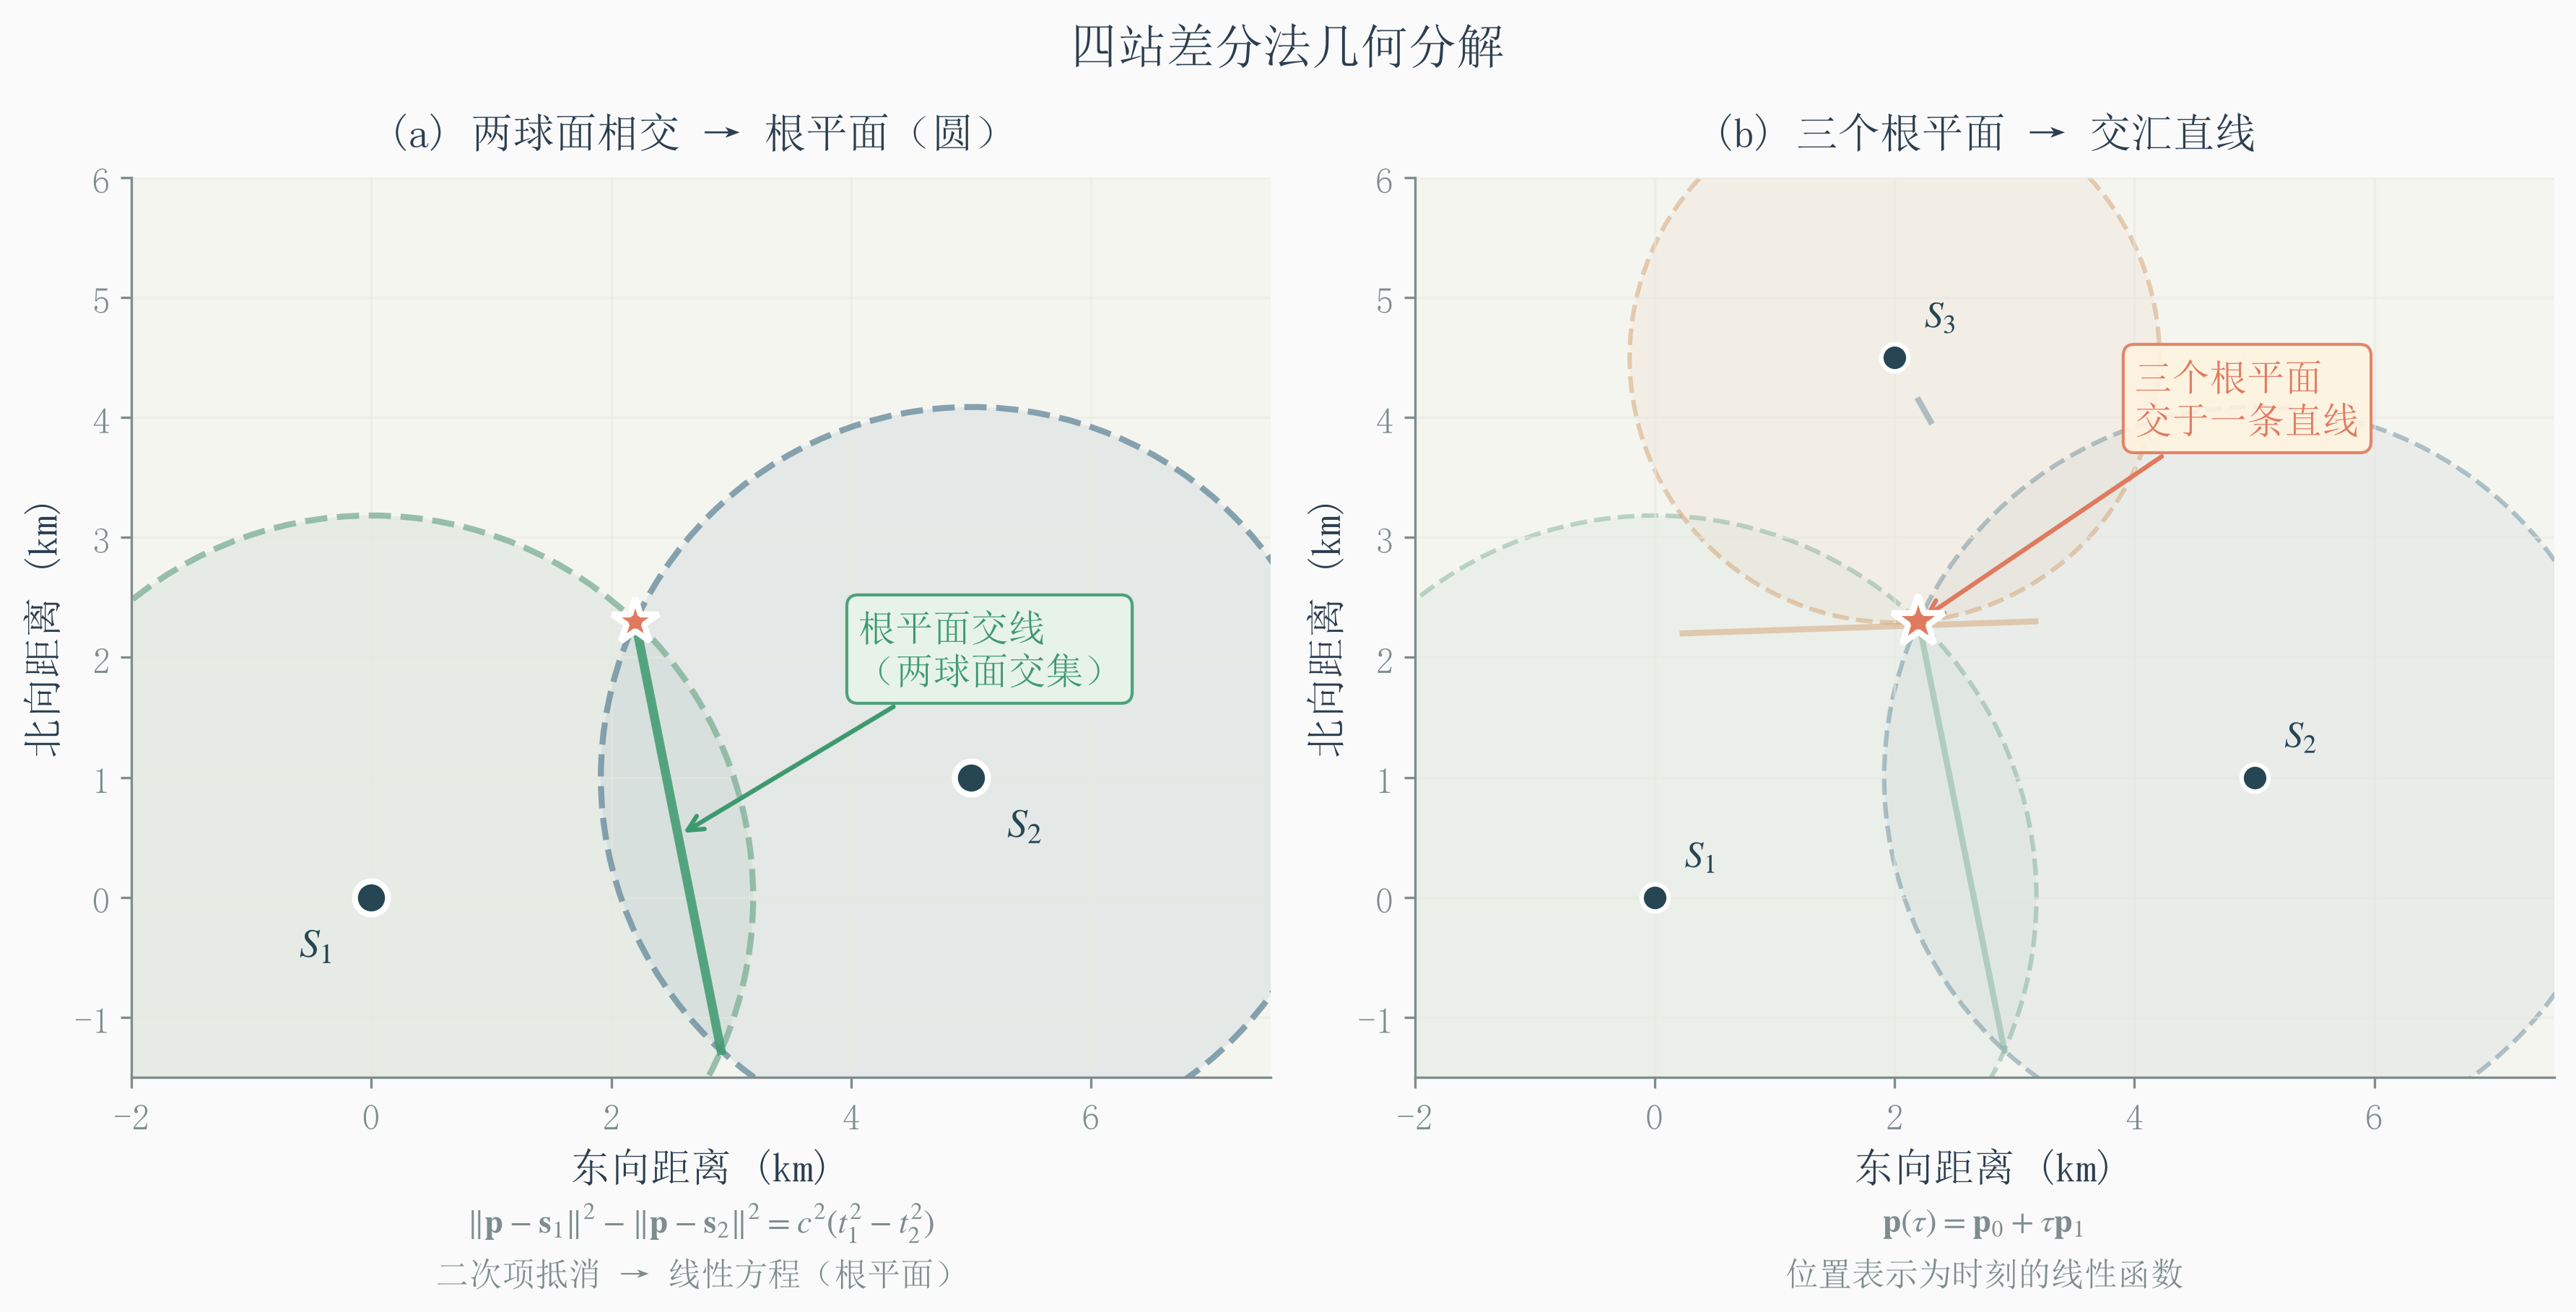
\includegraphics[width=1\textwidth]{output/figs/四站差分几何分解.png}
  \caption{四站差分法几何分解：根平面与交汇直线}\label{fig:diff-geo}
\end{figure}

 4台组合初筛可排除大量离谱的错解，却\textbf{不足以确认所有时间分别对应哪一个残骸}（即我们之前讨论过的冗余度问题），因此我们还需要以初筛结果为初值，用全部$n$台设备的TOA做\textbf{非线性最小二乘}精细化验真，计算全站RMSE。RMSE低于阈值（取$0.02$\,s）的候选进入下一层。这一步的鉴别力来自冗余观测，即错误关联不可能让全部设备的预测到达时刻同时撞上真实读数。

从通过验真的单事件候选中选出$n$个，使每台设备的$n$个读数被恰好各用一次，即解\textbf{精确覆盖问题}（exact cover），目标为最小化联合残差平方和$\sum_{j=1}^{n}\text{RMSE}_j^2$。

设备数由两个独立维度决定。可解性维度：4个未知量$(x,y,z,\tau)$需至少4个方程，故\textbf{理论下限为4台}。但4台只能解一个残骸，无法区分正确关联与不合常理的虚假关联，不具备任何冗余校验能力。
第5台设备可提供第一条冗余校验，使模型从可解跃升为可验证。用\textbf{位置精度因子（PDOP）}量化不同组合的定位精度：
\begin{equation}
  \text{PDOP}=\sqrt{\text{tr}\bigl[(\mathbf{H}^\top\mathbf{H})^{-1}_{1:3,1:3}\bigr]},
\end{equation}
其中$\mathbf{H}$为TOA雅可比矩阵。以问题三设备布局为基准，各组合在最坏残骸位置上的PDOP如表\ref{tab:pdop}所示。

\begin{table}[H]\centering
  \caption{不同设备组合的PDOP对比（单位：km/s）}\label{tab:pdop}
  \small
  \begin{tabular}{clccc}
    \toprule
    \textbf{设备数} & \textbf{组合} & \textbf{最坏PDOP} & \textbf{平均PDOP} & \textbf{评价} \\
    \midrule
    4 & ABEF & 3.110 & 2.305 & 最低可解配置，无冗余校验 \\
    5 & ABDEF & 2.979 & 2.187 & 新增一条残差校验，增益显著 \\
    6 & ABCDEF & 2.954 & 2.059 & 继续改善，边际收益变小 \\
    7 & ABCDEFG & 2.940 & 1.985 & 定位精度和容错更佳 \\
    \bottomrule
  \end{tabular}
\end{table}

ABCG组合虽满秩，但最坏PDOP高达$24.603$\,km/s，条件数$209.85$，几何构型极差，不应使用。
图\ref{fig:pdop-heat}进一步以热力图形式展示了4台（ABEF）与5台（ABDEF）组合在落区范围内的PDOP空间分布：4台时大片区域PDOP超过5\,km/s（橙红色），
边界处甚至超过10\,km/s；增加第5台后，PDOP整体下降约20\%，低PDOP区域明显扩大，中心区域落入2.5\,km/s以下（浅黄色）。
热力图直观印证了增加冗余检测站后精度显著提高。

\begin{figure}[H]
  \centering
  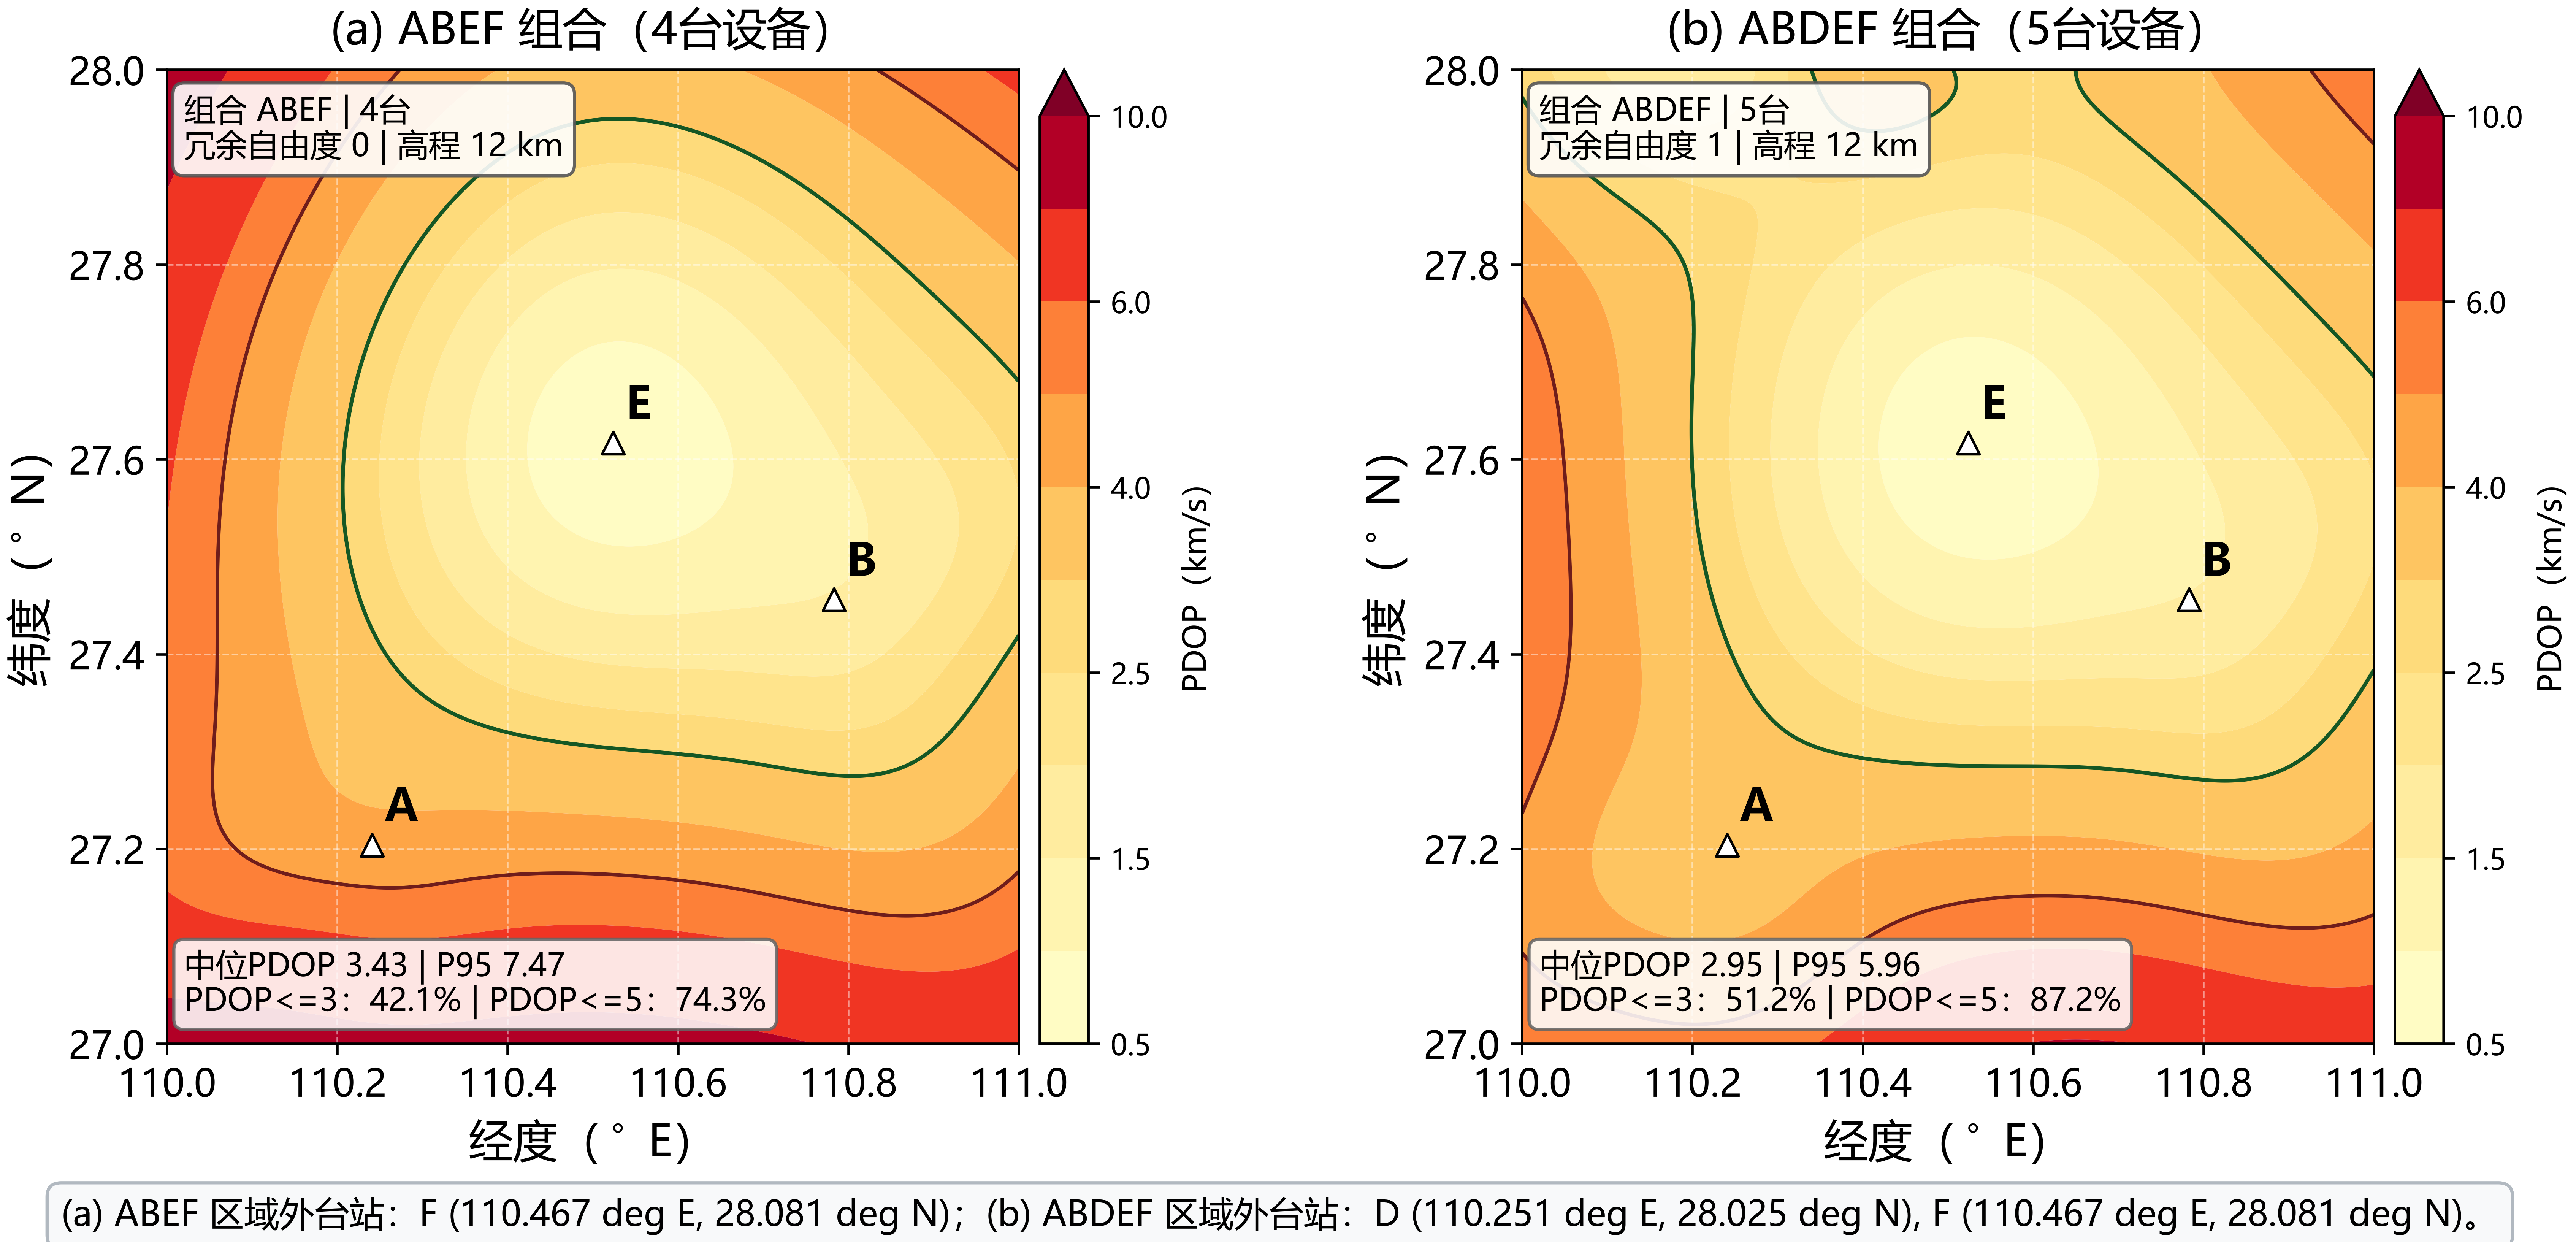
\includegraphics[width=0.92\textwidth]{output/figs/q2_pdop热力图.png}
  \caption{ABEF（4台）与ABDEF（5台）组合的PDOP空间分布对比}\label{fig:pdop-heat}
\end{figure}

综合以上分析，4个残骸的\textbf{理论下限为4台}，工程推荐\textbf{至少5台}；更多检测站引入的冗余度是鉴别不合常理的关联的可靠依据。

%================ 8 问题三 =================
\newpage
\section{问题三：四个残骸音爆位置与时刻的解算}

问题三给出7台设备的具体坐标和28个到达时刻数据。以设备A为参考点建立局部直角坐标系，所有计算在统一米-秒单位制下进行，声速$c=340$\,m/s。

\textbf{代入问题二模型}，求解流程如表\ref{tab:search}所示。

\begin{table}[H]\centering
  \caption{问题三搜索空间压缩过程}\label{tab:search}
  \small
  \begin{tabular}{ccc}
    \toprule
    \textbf{计算阶段} & \textbf{数量} & \textbf{说明} \\
    \midrule
    单事件组合总数 & $4^7=16384$ & 从7台设备各选一个读数 \\
    4站初筛、物理边界过滤后 & 1696 & 高程$\ge0$、音爆时刻早于所有观测 \\
    全站精细化后保留候选 & 4 & RMSE$<0.02$\,s且最大残差$<0.04$\,s \\
    精确覆盖组合 & \textbf{1} & 4个候选恰好完美覆盖28个读数，无冲突 \\
    \bottomrule
  \end{tabular}
\end{table}

4个残骸的最终解按音爆时刻排序如表\ref{tab:q3-result}所示。

\begin{table}[H]\centering
  \caption{问题三四残骸定位结果}\label{tab:q3-result}
  \small
  \begin{tabular}{ccccc}
    \toprule
    \textbf{残骸} & \textbf{经度(°E)} & \textbf{纬度(°N)} & \textbf{高程(km)} & \textbf{音爆时刻(s)} \\
    \midrule
    \#1 & 110.500001 & 27.309998 & 12.514 & 11.9999 \\
    \#2 & 110.499999 & 27.949998 & 11.529 & 13.0014 \\
    \#3 & 110.300000 & 27.650000 & 11.478 & 14.0000 \\
    \#4 & 110.699999 & 27.650000 & 13.468 & 15.0000 \\
    \bottomrule
  \end{tabular}
\end{table}


\begin{figure}[H]
  \centering
  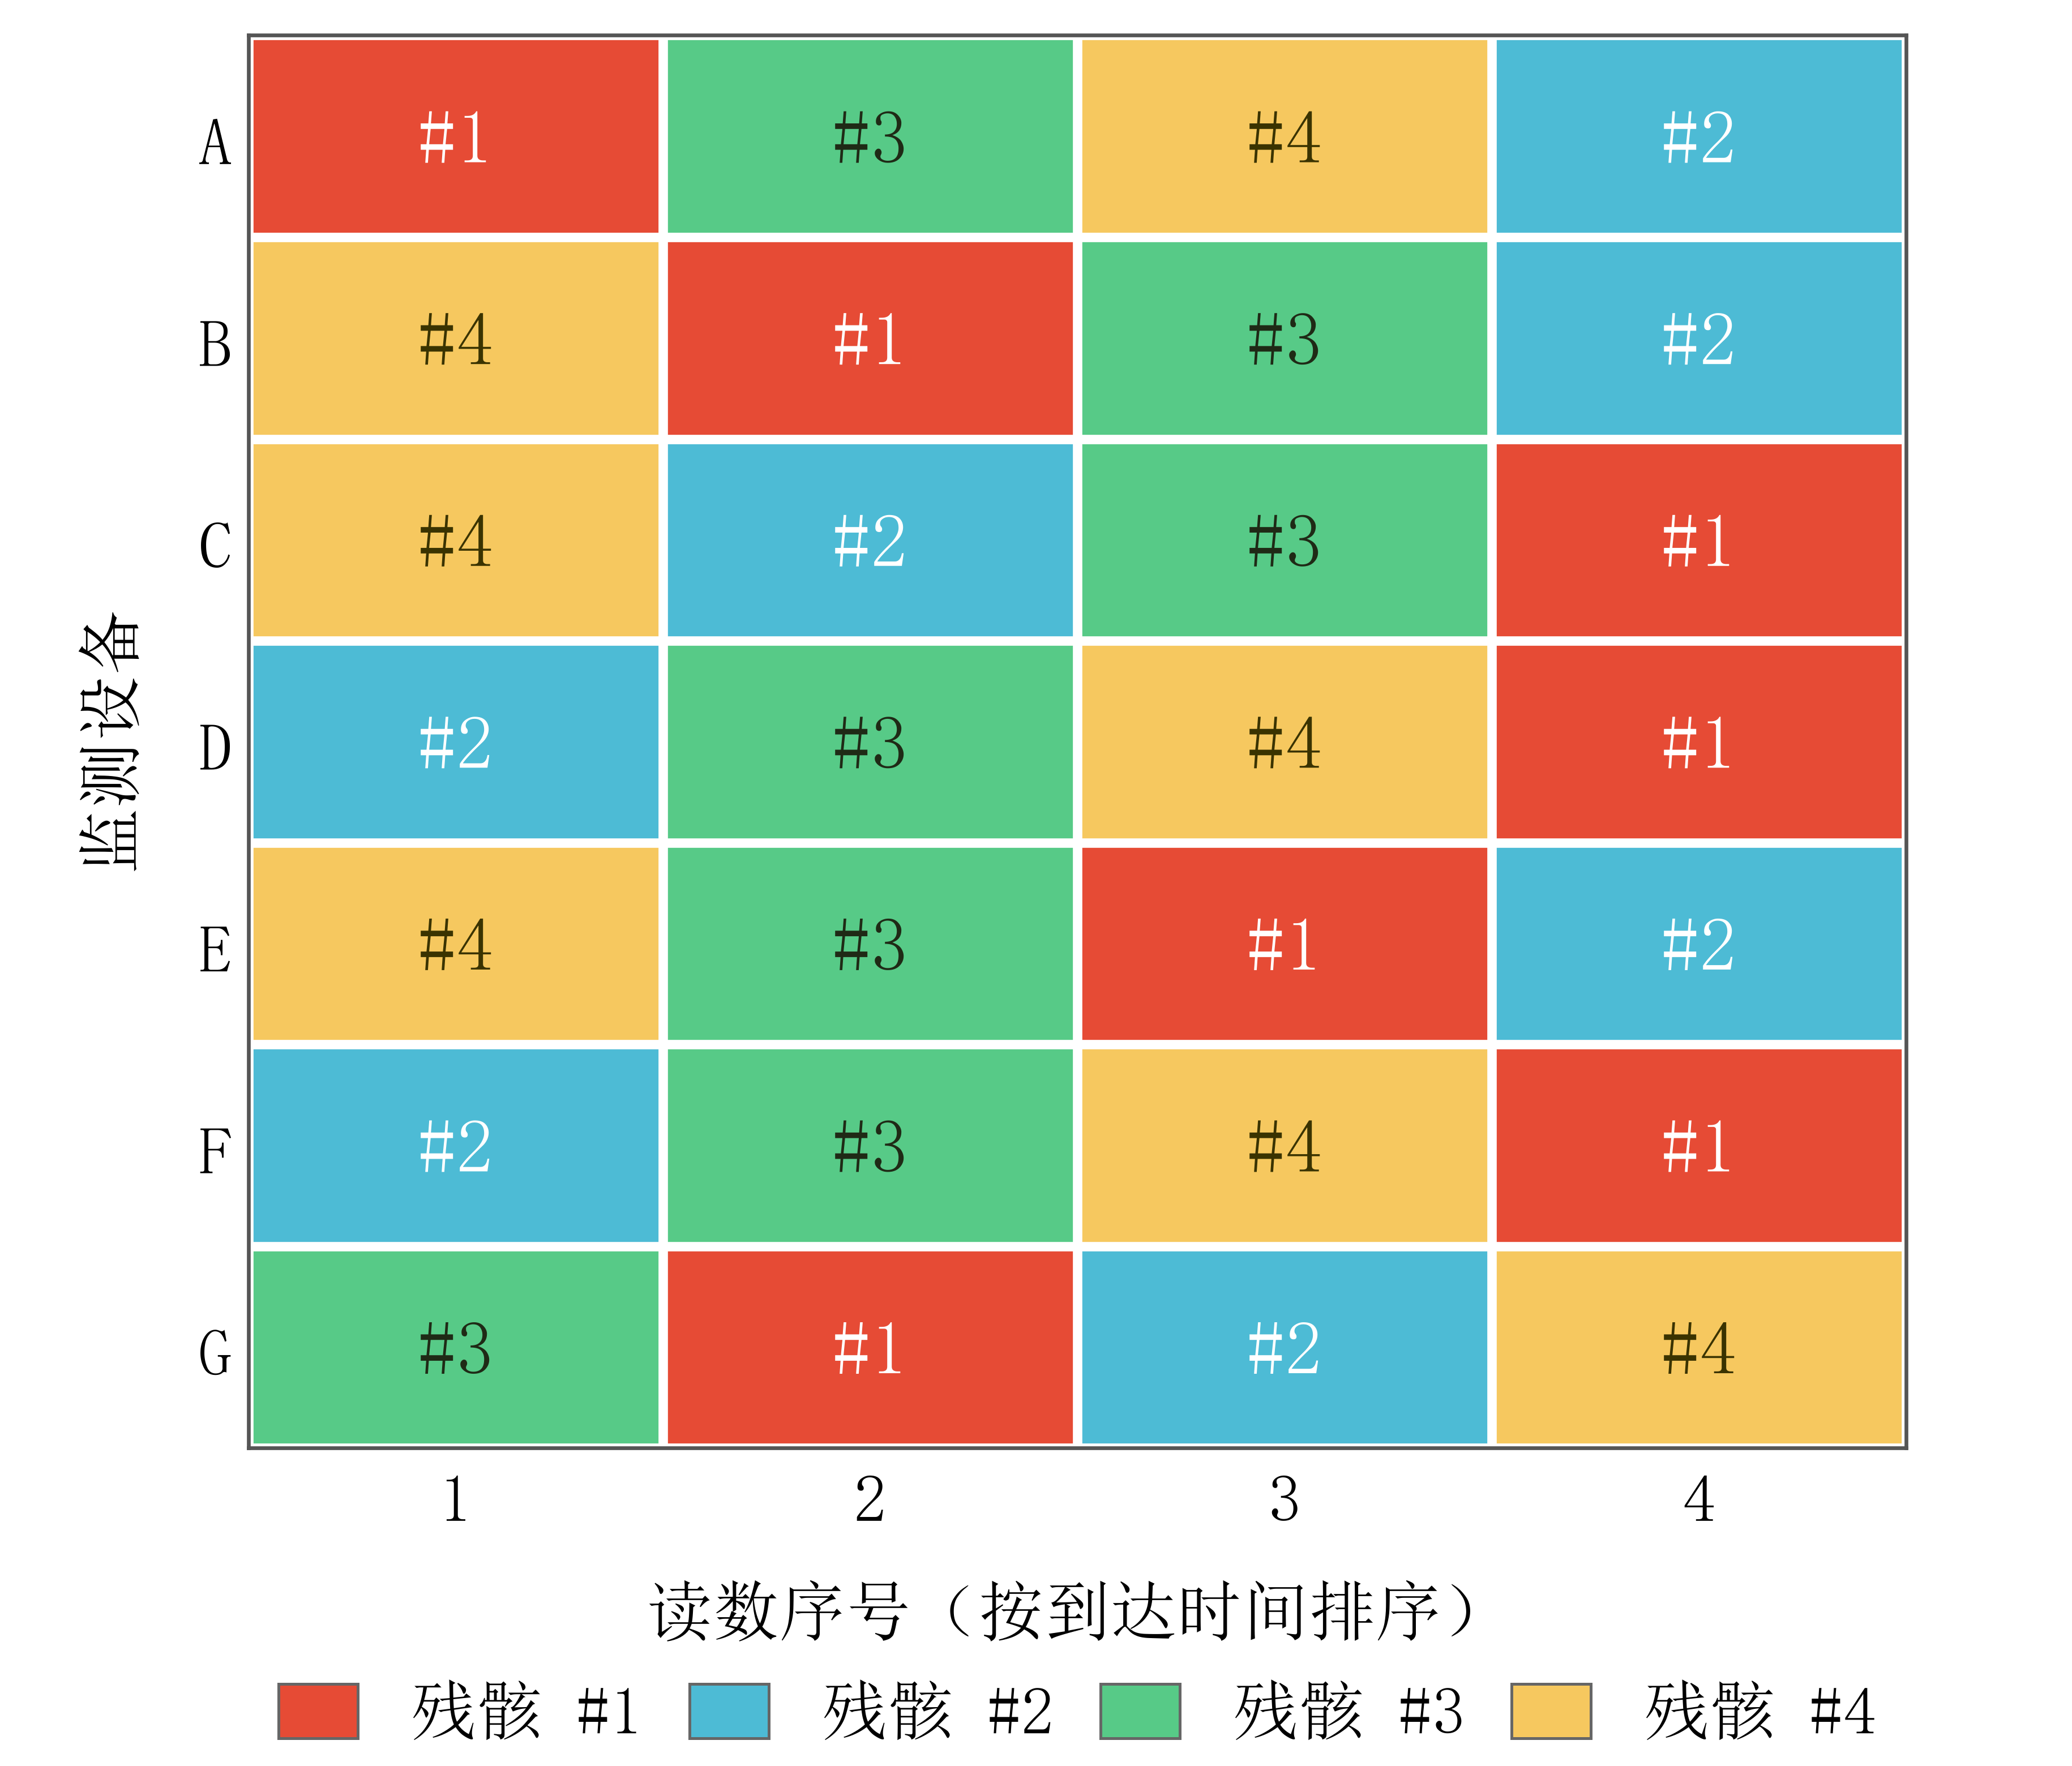
\includegraphics[width=0.7\textwidth]{output/figs/q3_设备读数与残骸关联矩阵.png}
  \caption{设备读数与残骸的关联矩阵}\label{fig:assoc-mat}
\end{figure}

图\ref{fig:assoc-mat}以热力图形式直观展示了每台设备4个读数与4个残骸（读数按时间先后编号1$\sim$4）的对应关系
。每台设备的4个色块恰好覆盖4种颜色（4个残骸各出现一次）。

4个音爆点在水平面上呈规则的十字对称分布（东西$\pm0.2°$、南北约$\pm0.32°$围绕中心$110.5°/27.63°$），时刻间隔接近1\,s，
数据内部一致性良好。图\ref{fig:q3-3d}以水平投影与高程剖面两种视角直观呈现了4个残骸的空间分布：左图为水平投影，
4个残骸（彩色圆点）分布在以$(110.5,27.65)$为中心的十字形区域内，高度从11.5\,km至13.5\,km不等；右图为沿南北和东西两个方向的正交高程剖面，
进一步确认各残骸处于跨音速飞行的典型高度区间，与接近地面的台站形成显著的垂直几何张角。

\begin{figure}[H]
  \centering
  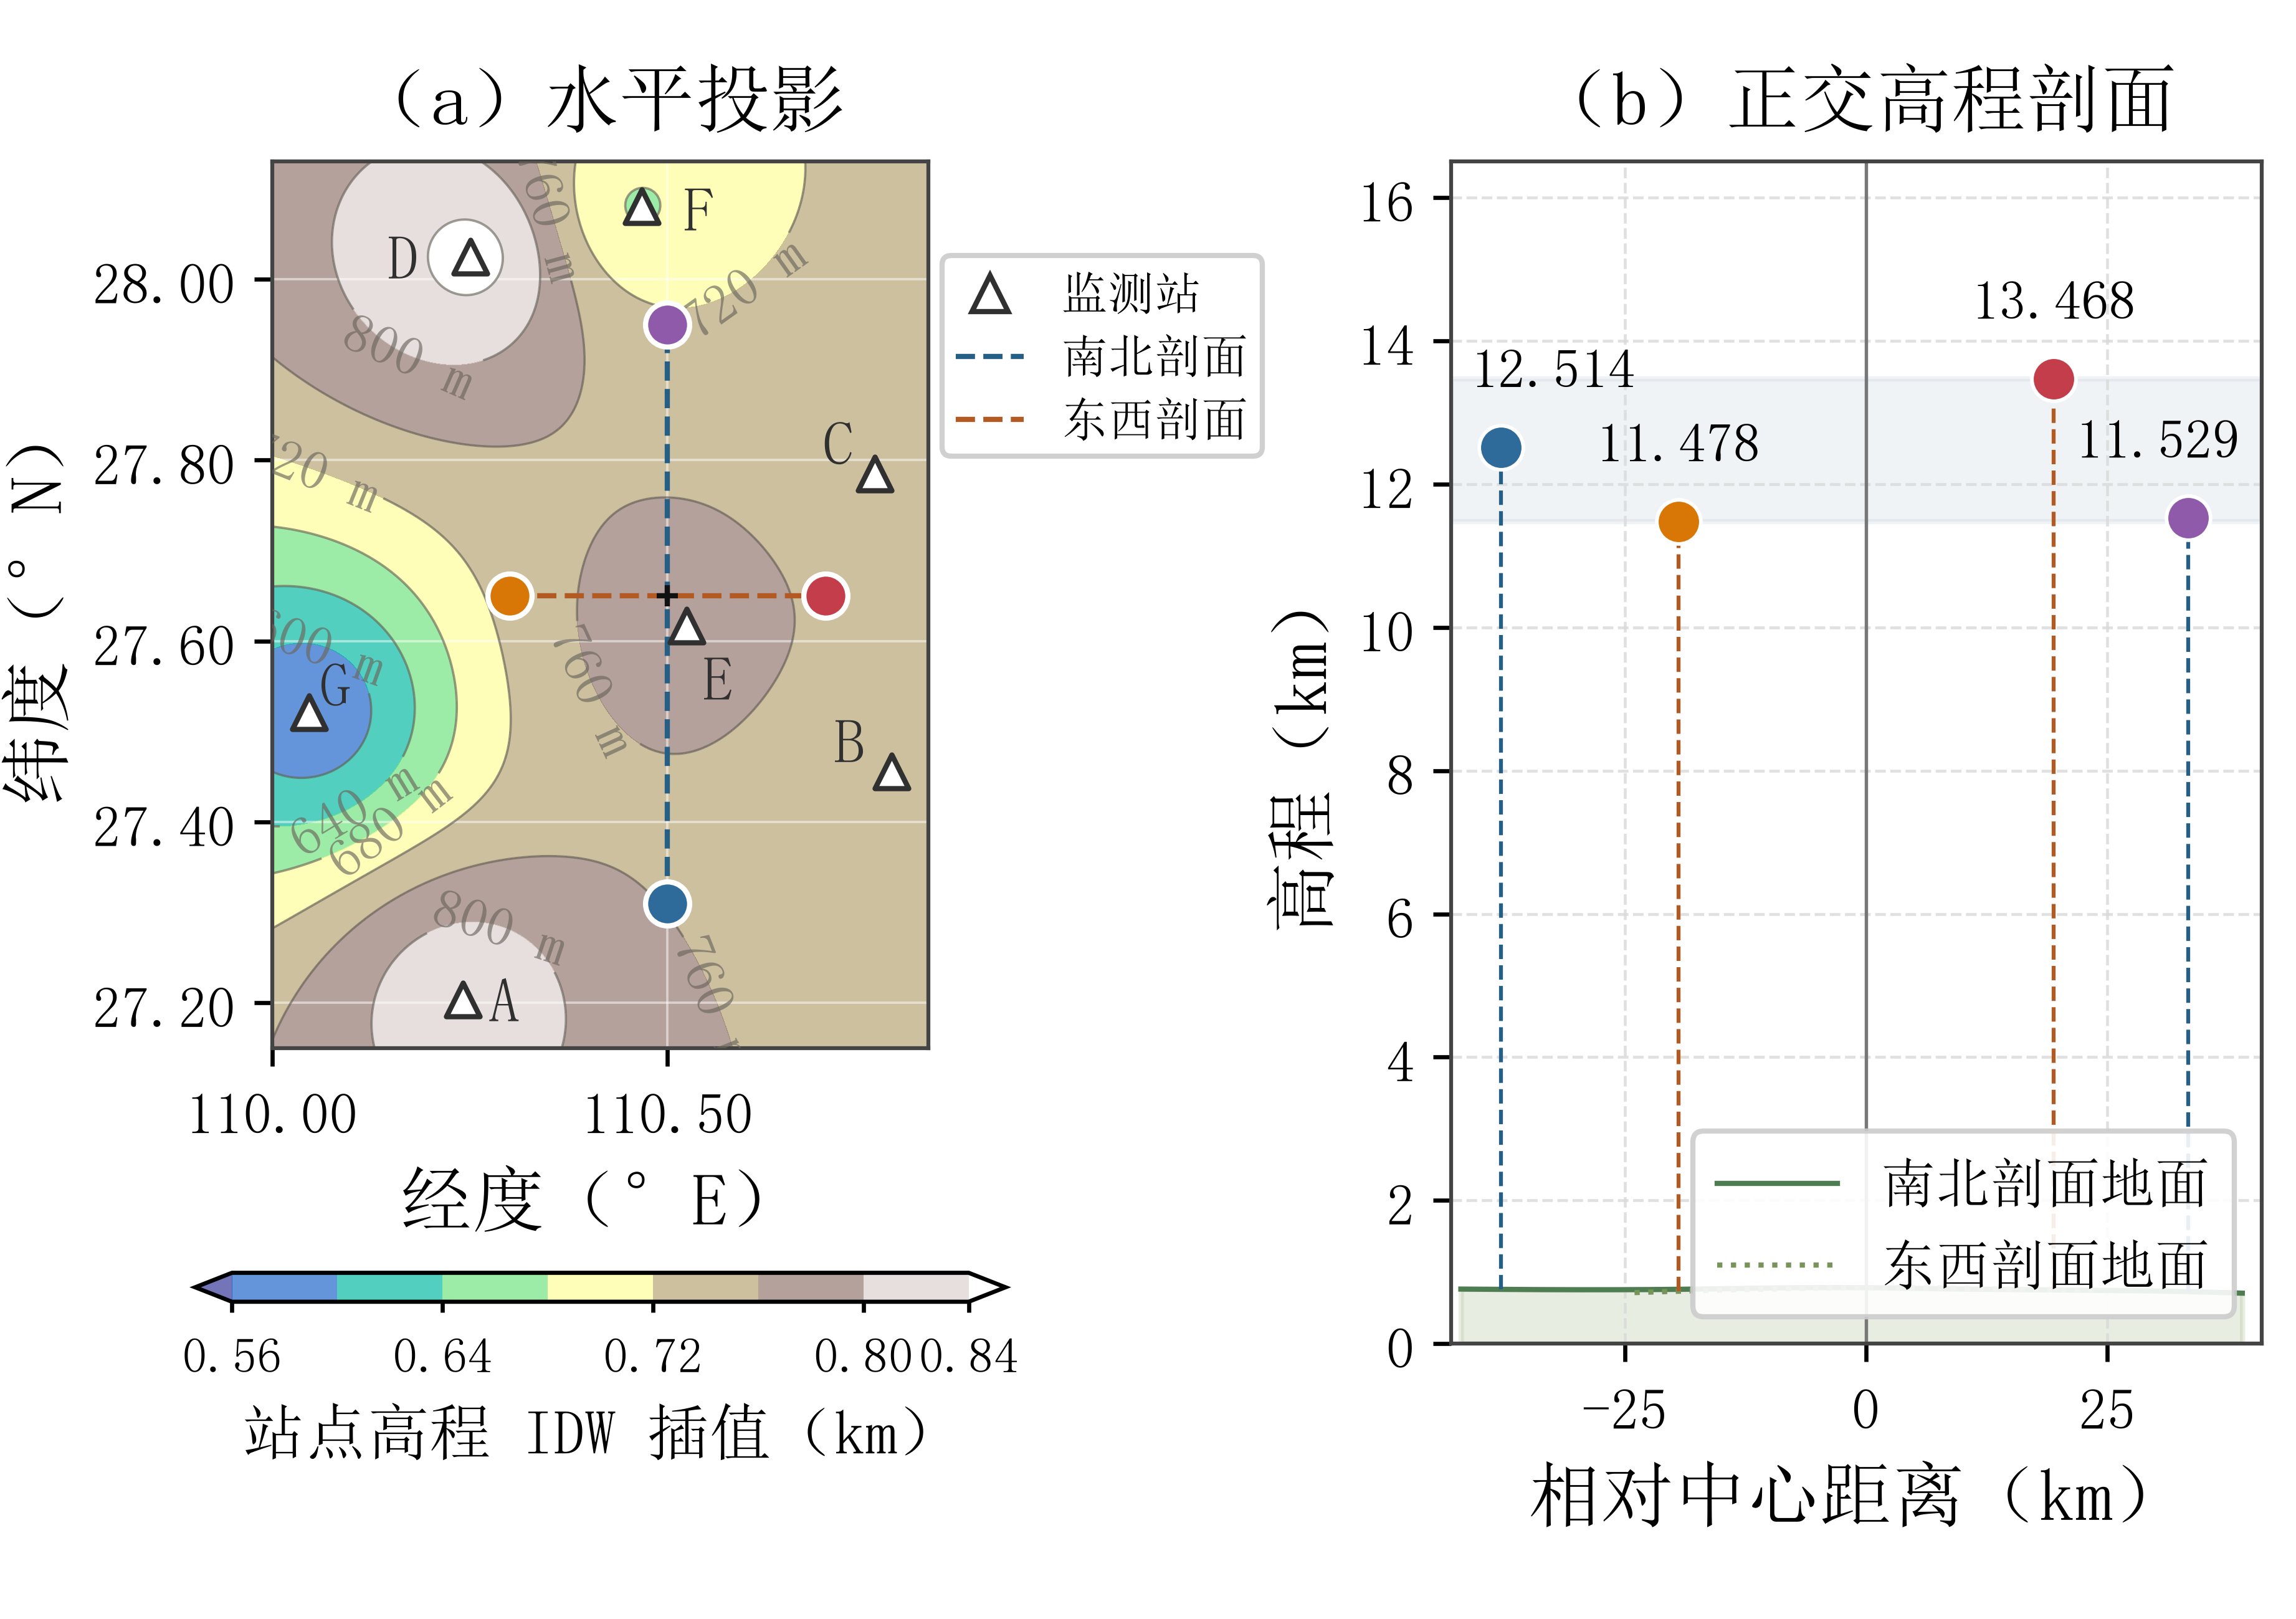
\includegraphics[width=0.92\textwidth]{output/figs/q3_水平投影与高程剖面.png}
  \caption{四个残骸的水平投影（左）与正交高程剖面（右）}\label{fig:q3-3d}
\end{figure}

4个音爆时刻为$11.9999$\,s、$13.0014$\,s、$14.0000$\,s、$15.0000$\,s，时间跨度$\Delta\tau=15.0000-11.9999=3.0001$\,s，满足题目不超过5\,s的要求。
本方案在求解过程中\textbf{未使用}5秒限制作为输入约束，但输出结果自然满足。这说明问题三的正确解不是由5秒的约束筛出来的；
即使把5秒限制加回模型作为硬约束，也不会改变结果。这说明模型的鉴别力来自\textbf{全部7台设备的联合TOA一致性}。


关联确定后对每个残骸做7站最小二乘精细化时的逐站残差（实测$-$预测到达时刻）如表\ref{tab:q3-residual}所示（单位：毫秒）。

\begin{table}[H]\centering
  \caption{问题三各残骸逐站残差（单位：ms）}\label{tab:q3-residual}
  \small
  \begin{tabular}{ccccccccc}
    \toprule
    \textbf{残骸} & \textbf{A} & \textbf{B} & \textbf{C} & \textbf{D} & \textbf{E} & \textbf{F} & \textbf{G} & \textbf{最大} \\
    \midrule
    \#1 & $+0.07$ & $-0.19$ & $+0.28$ & $-0.21$ & $+0.06$ & $+0.04$ & $-0.04$ & \textbf{0.28} \\
    \#2 & $+0.15$ & $-0.12$ & $+0.11$ & $+0.17$ & $+0.01$ & $-0.12$ & $-0.21$ & \textbf{0.21} \\
    \#3 & $+0.34$ & $-0.51$ & $+0.22$ & $-0.15$ & $+0.10$ & $+0.15$ & $-0.16$ & \textbf{0.51} \\
    \#4 & $-0.23$ & $+0.16$ & $-0.16$ & $-0.01$ & $+0.04$ & $+0.12$ & $+0.08$ & \textbf{0.23} \\
    \bottomrule
  \end{tabular}
\end{table}

全部28个残差落在$\pm0.6$\,ms以内，RMS仅$0.18$\,ms，折合成距离不到$0.2$\,m。残差呈随机抖动，无系统性符号偏向；
各站最大残差分布较均匀，没有某站显著偏大。这说明\textbf{7台设备全部可靠，无需剔除}。冗余度$r=7-4=3$全部转化为精度提升，无需排除异常站。
若某站存在异常，其读数\textbf{在关联验证阶段就匹配不上}任何合理残骸假设的预测；即使混进关联，精细化后该站残差也会\textbf{显著大于其他站}。设备均通过了两层模型的检验。



%================ 9 问题四 =================
% ================= 9 问题四 =================
\section{问题四：含随机时间误差的模型修正与布站设计}

问题四要求我们在设备记录时间存在$0.5$\,s随机误差的情形下，修正问题二的关联--定位模型，给出算例并分析误差；若时间误差无法降低，则需设计新的监测方案，实现误差小于$1$\,km的空中精准定位，并自行模拟台站位置与观测数据加以验证。

设各读数的计时误差$\varepsilon_{ik}\sim U(-\Delta,+\Delta)$，$\Delta=0.5$\,s，各站各读数相互独立，标准差$\sigma_t=\Delta/\sqrt{3}\approx0.289$\,s。折算成距离，单站测距不确定性达$\pm170$\,m，比问题三数据自身的自洽水平（亚毫秒量级）高出约三个数量级——问题二模型在这样的误差环境下\textbf{无法直接沿用}，必须修正。

问题二模型的鉴别逻辑是：枚举$4^7=16384$种单事件组合，正确关联在全站上的RMSE接近零（验真阈值取$0.02$\,s），
而错误关联不可能让7台设备的预测时刻同时撞上真实读数。叠加$\pm0.5$\,s噪声后，这套逻辑在两个环节上失效：
\textbf{1.阈值失效},正确关联的残差被抬升到噪声本身的量级（约$\pm0.3$\,s），继续沿用$0.02$\,s的阈值，100次实验中有79次连4个候选都凑不齐，说明
\textbf{真解被误杀}；其二，\textbf{组合退化}——初筛结果由4站差分方程生成，噪声经几何放大后，固定一个4台组合约有$31\%$的概率给出偏离真解过远组合，
正确组合在初筛阶段即被丢弃。为此，我们对模型做三项修正。

\textbf{1.验真阈值的统计标定。}阈值不再人为指定，而是用蒙特卡洛模拟把噪声传播到残差域，分别标定正确关联与错误关联的残差分布：
正确关联（240次实验）精化后RMSE的中位数为$0.142$\,s、99\%分位为$0.30$\,s，最大残差的99\%分位为$0.54$\,s；错误关联经4参数最小二乘拟合摊薄后，
最优者的RMSE最小值也有$0.43$\,s。据此取\textbf{严格阈值RMSE$<0.55$\,s且max$|$残差$|<0.65$\,s}，正确关联通过率超过$99\%$，
绝大多数错误关联被拦在门外。需要坦诚的是，鉴别间隙变窄了：无噪声时是$0.0002$\,s与数秒的天壤之别，
现在是$0.30$\,s对$0.43$\,s这正是下一项容错机制存在的理由。

\textbf{2.多个初筛组合批量解析。}不再依赖单一4台组合，而是预计算\textbf{条件数最低的4台组合}（DEFG、ABDG、ACDG、ADEG），
任一组通过物理约束初筛即送入精细化；同时将枚举组合--解线性方程组--解二次方程--全站初筛整条链路向量化，单次求解效率大幅提升，
使数百次蒙特卡洛实验在算力上可行。修正后正确关联的4台组合捕获率由$69\%$提升至\textbf{$240/240$}。

\textbf{3.分级阈值与剩余读数补全的容错机制。}针对变窄的鉴别间隙增设两级兜底：第一级按严格阈值枚举候选并执行精确覆盖，
约$99\%$的实验在此直接得到唯一覆盖；若个别正确关联因极端噪声被误杀、候选只剩3个，则这3个候选已锁定7站共21个读数，
\textbf{每站恰好剩下的1个未用读数在物理上必然属于第4个残骸}，直接将其送入精细化并用宽阈值（RMSE$<0.9$\,s）验证即可。
300次蒙特卡洛实验中，298次走第一级、2次触发补全，\textbf{关联成功率$300/300$，无一失败、无一混淆}。

修正后的求解流程为：批量解析4个4台组合$\to$初筛$\to$精细化$\to$统计阈值验真$\to$精确覆盖或剩余读数补全。与问题二模型相比，
\textbf{框架骨架完全保留}——TOA方程、精确覆盖约束、物理与空间边界、全站联合残差均未改动，修正集中在误差环境下阈值从哪来、组合退化怎么办、
边界情形如何兜底三处。

对问题三数据叠加一组$U(-0.5,+0.5)$\,s噪声（固定随机种子，结果可复现），修正模型输出候选4个、覆盖唯一，定位结果如表\ref{tab:q4-single}所示。

\begin{table}[H]\centering
  \caption{叠加随机误差后的单次算例定位结果}\label{tab:q4-single}
  \small
  \begin{tabular}{ccccccc}
    \toprule
    \textbf{残骸} & \textbf{经度(°E)} & \textbf{纬度(°N)} & \textbf{高程(km)} & \textbf{音爆时刻(s)} & \textbf{3D误差(m)} & \textbf{时刻误差(ms)} \\
    \midrule
    \#1 & 110.4995 & 27.3105 & 12.278 & 12.206 & 247 & 206 \\
    \#2 & 110.4983 & 27.9485 & 10.996 & 13.685 & 582 & 683 \\
    \#3 & 110.3002 & 27.6501 & 11.644 & 13.884 & 167 & 116 \\
    \#4 & 110.7010 & 27.6511 & 13.639 & 14.674 & 231 & 326 \\
    \bottomrule
  \end{tabular}
\end{table}

关联正确，4个残骸全部落在真值$600$\,m以内。单次算例说明``能用''，但说明不了统计规律，我们进一步做\textbf{300次独立噪声实现的蒙特卡洛实验}，结果如表\ref{tab:q4-mc7}所示。

\begin{table}[H]\centering
  \caption{7台现状下蒙特卡洛误差统计（300次）}\label{tab:q4-mc7}
  \small
  \begin{tabular}{lcccc}
    \toprule
    \textbf{指标} & \textbf{均值} & \textbf{中位数} & \textbf{95\%分位} & \textbf{最大值} \\
    \midrule
    水平误差 & 135\,m & 108\,m & 331\,m & 635\,m \\
    高程误差 & 455\,m & 354\,m & \textbf{1196\,m} & 1964\,m \\
    3D误差 & 486\,m & 374\,m & \textbf{1224\,m} & 2018\,m \\
    时刻误差 & 523\,ms & 394\,ms & 1443\,ms & 2688\,ms \\
    \bottomrule
  \end{tabular}
\end{table}

3D误差超过$1$\,km的实验占\textbf{$10.4\%$}——7台现状在$\pm0.5$\,s噪声下\textbf{不满足}误差小于$1$\,km的要求。误差分布呈现明显的方向性：水平方向95\%分位仅$331$\,m，而高程方向高达$1196$\,m，瓶颈独在高程。

这一方向性可由观测几何解释。把定位想象成``从多个方向拉皮筋确定一个点''：皮筋交汇的角度越开，点的位置越稳。7台设备全部贴在地面（高程575$\sim$850\,m），而音爆点在$11\sim13$\,km高空，所有观测方向都从下往上、挤在一个朝天的小锥角里。水平面内设备环绕残骸分布，拉得开角度，故水平误差只有三百来米；垂直方向上，到达时刻对高程的灵敏度为$\partial t/\partial z=(z-z_i)/(c\,d_i)$，音爆点\textbf{正下方}的站灵敏度接近$1/c$（最强），远处站趋近于零，而7台设备离残骸地面投影都有$20\sim70$\,km，\textbf{没有一台在近正下方}，高程方向几乎无独立约束，其误差与音爆时刻$\tau$的误差互相耦合（高程多$1.2$\,km与时刻晚$1.4$\,s在数据上几乎不可区分）。这不是算法问题，而是\textbf{几何配置问题}——再聪明的算法也榨不出数据里没有的信息，这直接指明了下一步的方向。

既然时间误差本身无法降低（$\sigma_t\approx0.289$\,s固定），能动的只有监测设备网。定位精度由\textbf{位置精度因子（PDOP）}决定，$\sigma_{\mathrm{3D}}\approx\mathrm{PDOP}\times\sigma_t$。目标``95\%分位3D误差小于$1$\,km''约需$\sigma_{\mathrm{3D}}\lesssim0.5$\,km，即\textbf{PDOP$\lesssim1.73$\,km/s}。以此为精度预算，我们对若干候选布局做PDOP核算，结果如表\ref{tab:q4-pdop}所示。

\begin{table}[H]\centering
  \caption{候选监测设备网布局的PDOP精度预算}\label{tab:q4-pdop}
  \small
  \begin{tabular}{lcccc}
    \toprule
    \textbf{布局} & \textbf{台数} & \textbf{最坏PDOP(km/s)} & \textbf{预估}$\sigma_{\mathrm{3D}}$\textbf{(m)} & \textbf{判断} \\
    \midrule
    原7台 & 7 & 2.940 & 849 & 不足 \\
    7台+外环8台（45\,km） & 15 & 1.852 & 535 & 勉强，余量太小 \\
    7台+中心1台+外环8台 & 16 & 1.456 & 420 & 边缘 \\
    \textbf{7台+中心1台+内环4台（15\,km）+外环8台} & \textbf{20} & \textbf{0.981} & \textbf{283} & \textbf{推荐} \\
    7台+内环6台+外环10台 & 23 & 0.801 & 231 & 更优但多3台 \\
    \bottomrule
  \end{tabular}
\end{table}

最终方案为\textbf{原7台不动，新增13台，共20台}，两个设计要点都直接回应上文的误差归因：其一，\textbf{在落区正下方设中心站}，给高程方向补上最强的灵敏度，仅加这1台即可使PDOP再降$21\%$，是压制高程误差的关键；其二，\textbf{分层环绕}，内环（半径15\,km）提供近距大角度观测，外环（半径45\,km）提供长基线包络，随机误差随独立观测数按$1/\sqrt{m}$被进一步平均。新增台站坐标如表\ref{tab:q4-stations}所示。

\begin{table}[H]\centering
  \caption{新增13台监测设备坐标（原7台保持不动）}\label{tab:q4-stations}
  \small
  \begin{tabular}{ccccc}
    \toprule
    \textbf{新增设备} & \textbf{经度(°E)} & \textbf{纬度(°N)} & \textbf{高程(m)} & \textbf{所属环} \\
    \midrule
    N01 & 110.5000 & 27.6500 & 800 & 中心（落区正下方） \\
    N02$\sim$N05 & 110.6090\,/\,110.3910 & 27.7453\,/\,27.5547 & 750 & 内环，半径15\,km \\
    N06$\sim$N13 & 110.9273\,/\,110.6770\,/\,110.3230\,/\,110.0727 & 27.8048\,/\,28.0237\,/\,27.4952\,/\,27.2763 & 750 & 外环，半径45\,km \\
    \bottomrule
  \end{tabular}
\end{table}

台数从7增至20后，直接枚举关联需要$4^{20}\approx1.1\times10^{12}$次，不可行。但关联的判别力只需要一个几何构型良好的7台子网，因此我们采用\textbf{两阶段求解策略}：\textbf{阶段一}，用原7台走修正模型的``枚举--验真--覆盖''流程，得到4个粗解，关联正确率已由上文的蒙特卡洛实验证明；\textbf{阶段二}，用粗解预测全部20台的到达时刻，按``宽窗口（6\,s）最近邻关联$\to$20站联合最小二乘精细化$\to$紧窗口（1.5\,s）重关联$\to$再精细化''迭代，各站相邻残骸读数的最小间隔为$2.97$\,s，精细化后预测偏差小于$1$\,s，紧窗口下不会错配。这与问题二模型的精神一致：枚举只需发生在\textbf{最小充分子网}上，新增设备以``预测--匹配''方式低成本吸收。

最后，按题目要求用问题三的4个定位结果作真值，正向生成20台的无噪声到达时刻（每站4个，按时间先后编号），叠加$U(-0.5,+0.5)$\,s噪声后用两阶段修正模型盲解反演。单次算例（固定随机种子）如表\ref{tab:q4-single20}所示，300次蒙特卡洛统计如表\ref{tab:q4-mc20}所示。

\begin{table}[H]\centering
  \caption{20台加密监测设备网单次算例反演结果}\label{tab:q4-single20}
  \small
  \begin{tabular}{cccccc}
    \toprule
    \textbf{残骸} & \textbf{经度(°E)} & \textbf{纬度(°N)} & \textbf{高程(km)} & \textbf{音爆时刻(s)} & \textbf{3D误差(m)} \\
    \midrule
    \#1 & 110.5005 & 27.3090 & 13.077 & 11.322 & 575 \\
    \#2 & 110.5001 & 27.9500 & 11.593 & 12.908 & 66 \\
    \#3 & 110.2994 & 27.6506 & 11.201 & 14.079 & 292 \\
    \#4 & 110.7008 & 27.6502 & 13.379 & 15.033 & 124 \\
    \bottomrule
  \end{tabular}
\end{table}

\begin{table}[H]\centering
  \caption{20台加密监测设备网蒙特卡洛误差统计（300次，并与7台对比）}\label{tab:q4-mc20}
  \small
  \begin{tabular}{lccccc}
    \toprule
    \textbf{指标} & \textbf{均值} & \textbf{中位数} & \textbf{95\%分位} & \textbf{最大值} & \textbf{7台95\%分位对比} \\
    \midrule
    水平误差 & 60\,m & 55\,m & 129\,m & 216\,m & 331\,m（$\downarrow61\%$） \\
    高程误差 & 169\,m & 137\,m & 449\,m & 797\,m & 1196\,m（$\downarrow62\%$） \\
    3D误差 & 187\,m & 149\,m & \textbf{457\,m} & \textbf{810\,m} & 1224\,m（$\downarrow63\%$） \\
    时刻误差 & 208\,ms & 163\,ms & 556\,ms & 868\,ms & 1443\,ms（$\downarrow61\%$） \\
    \bottomrule
  \end{tabular}
\end{table}

反演验证表明：\textbf{关联成功率$300/300$}（含阶段一的2次容错补全），无关联混淆；\textbf{3D误差超过$1$\,km的比例为$0.00\%$}，最大值$810$\,m、95\%分位$457$\,m，误差小于$1$\,km的目标达成且留有约一倍余量；实测误差水平与PDOP精度预算（$\sigma_{\mathrm{3D}}\approx283$\,m）高度吻合，说明该预算可以直接指导监测设备网设计，做到``先算后建''，无需事后补救。

综上，问题四的结论为：$\pm0.5$\,s计时误差下，问题二模型的框架不必推翻，经\textbf{阈值统计标定、多初筛组合批量解析、分级容错}三项修正后，关联成功率保持\textbf{$100\%$}；但7台现状的3D误差95\%分位达$1224$\,m、$10.4\%$的实验超过$1$\,km，瓶颈在\textbf{高程方向}，根源是台站全在地面、垂直几何张角不足的几何配置问题；将监测设备网加密至\textbf{20台}（新增中心1台、内环4台、外环8台），配合``子网定关联、全网提精度''的两阶段策略，3D误差95\%分位降至\textbf{$457$\,m}、最大\textbf{$810$\,m}，稳定满足误差小于$1$\,km的定位要求。

%================ 10 模型的分析与检验 =================
\section{模型的分析与检验}

问题四的修正模型与加密监测设备网方案均建立在``计时误差服从$U(-0.5,+0.5)$\,s、各读数相互独立''的标称假设上。本节刻意打破这些假设，考察当误差顶满边界、超出标称水平或出现设备粗差时模型是否依然稳健。全部检验\textbf{不修改模型、不调整参数}，仅改变输入数据的噪声结构，每项检验均在7台现状与20台加密监测设备网两种配置下进行。

\subsection{误差分布形态检验}

均匀分布的大部分实现落在$\pm0.3$\,s以内，而两点分布让每个读数都顶满$\pm0.5$\,s边界，等效标准差$\sigma=0.5$\,s，比标称情形恶劣$73\%$，是``$\pm0.5$\,s误差''假设下统计性质最坏的情形。检验结果如表\ref{tab:test-bimodal}所示。

\begin{table}[H]\centering
  \caption{两点分布（每读数独立取$\pm0.5$\,s）下的模型表现}\label{tab:test-bimodal}
  \small
  \begin{tabular}{lcc}
    \toprule
    \textbf{指标} & \textbf{7台} & \textbf{20台} \\
    \midrule
    关联成功 & \textbf{300/300} & \textbf{300/300} \\
    水平误差95\%分位 & 559\,m & 217\,m \\
    高程误差95\%分位 & 2176\,m & 776\,m \\
    3D误差95\%分位\,/\,最大值 & \textbf{2206\,m\,/\,3157\,m} & \textbf{795\,m\,/\,1455\,m} \\
    3D误差超过1\,km比例 & \textbf{30.8\%} & \textbf{1.58\%} \\
    \bottomrule
  \end{tabular}
\end{table}

有两点值得记录。其一，\textbf{容错机制从兜底变成了主力}：严格阈值按均匀分布标定，在两点分布下误杀率升至$76\%$，300次实验中有229次靠剩余读数补全才完成关联，且无一出错，说明补全机制足以独立承担主力角色。其二，20台加密监测设备网的95\%分位$795$\,m仍达标，但最大值$1455$\,m出现个别超标，标称情形下的精度余量被边界噪声吃掉——\textbf{监测设备网加密的冗余设计买的不是更准的平均值，而是更窄的坏情形尾巴}。

\subsection{噪声幅度灵敏度检验}

将噪声界$\Delta$从$0.1$\,s递增至$1.0$\,s（每档40$\sim$100次蒙特卡洛），刻画模型性能随噪声水平的完整退化曲线，结果如表\ref{tab:test-delta}所示。

\begin{table}[H]\centering
  \caption{噪声幅度扫描（7台，$U(-\Delta,+\Delta)$）}\label{tab:test-delta}
  \small
  \begin{tabular}{cccccc}
    \toprule
    $\Delta$\textbf{(s)} & \textbf{关联成功} & \textbf{3D误差95\%分位} & \textbf{最大值} & \textbf{超1\,km占比} & \textbf{求解模式} \\
    \midrule
    0.1 & 100/100 & 253\,m & 436\,m & 0.0\% & 严格阈值 \\
    0.2 & 100/100 & 523\,m & 762\,m & 0.0\% & 严格阈值 \\
    0.3 & 100/100 & 833\,m & 1449\,m & 1.5\% & 严格阈值 \\
    0.4 & 100/100 & 1010\,m & 1669\,m & 5.5\% & 严格阈值 \\
    0.5 & 100/100 & 1233\,m & 1791\,m & 9.0\% & 严格阈值 \\
    0.6 & 60/60 & 1481\,m & 2060\,m & 17.1\% & 严格为主 \\
    0.7 & 60/60 & 1684\,m & 3599\,m & 23.8\% & 补全占40\% \\
    \textbf{0.8} & \textbf{37/40} & 1917\,m & 3735\,m & 31.1\% & 补全为主，首现失败 \\
    0.9 & 36/40 & 2197\,m & 3290\,m & 33.3\% & 补全占75\% \\
    1.0 & \textbf{30/40} & 2213\,m & 3484\,m & 39.2\% & 失败率25\% \\
    \bottomrule
  \end{tabular}
\end{table}

扫描曲线识别出三个临界点。\textbf{精度崩溃点$\Delta\approx0.4$\,s}：95\%分位在此越过$1$\,km，印证了7台在标称的$0.5$\,s下本就不达标、问题出在几何而非算法的结论。\textbf{关联崩溃点$\Delta\approx0.8$\,s}：按$\sigma\approx0.3$\,s标定的两级阈值开始系统性误杀正确关联；而$\Delta\leq0.6$\,s时关联成功率保持$100\%$，说明\textbf{阈值设计留有约$60\%$的噪声超调余量}。此外，$\Delta\leq0.6$\,s区间内95\%分位误差与$\Delta$近似成正比（253$\to$523$\to$833$\to$1010$\to$1233$\to$1481\,m），符合$\sigma_{\mathrm{3D}}\approx\mathrm{PDOP}\times\sigma_t$的线性精度预算，\textbf{在崩溃点之前模型行为完全可预测}，无非线性失稳迹象。20台加密监测设备网在$\Delta=1.0$\,s时关联成功$47/60$，通过者的95\%分位为$1056$\,m，失败集中在阶段一的7台子网关联环节，而非全网几何。

\subsection{系统偏差检验}

分两种典型形态检验系统性误差。第一种是\textbf{全体同号偏差}：所有读数同时偏移$\pm0.5$\,s，模拟时钟零点的整体平移。此时3D误差仅\textbf{$0.1\sim0.2$\,m}，偏差被每个残骸的音爆时刻参数$\tau$完全吸收——TOA方程中只有站间时间差携带几何信息。这说明模型对工程上最常见的时钟同步误差\textbf{天然免疫}，是最温和的极端情形。

第二种是\textbf{台站级系统偏差}：每台设备的4个读数同向偏移$\pm0.5$\,s，模拟设备级标定偏差，这是无法被$\tau$吸收、也不能被$1/\sqrt{m}$平均掉的误差形态。7台穷举全部$2^7=128$种符号模式，20台随机抽60种，结果如表\ref{tab:test-sysbias}所示。

\begin{table}[H]\centering
  \caption{台站系统偏差（每站读数同号$\pm0.5$\,s）下的模型表现}\label{tab:test-sysbias}
  \small
  \begin{tabular}{lcccc}
    \toprule
    \textbf{监测设备网} & \textbf{失败/混淆} & \textbf{3D误差中位数} & \textbf{3D误差95\%分位} & \textbf{超1\,km占比} \\
    \midrule
    7台（穷举128种） & \textbf{0} & 1520\,m & 2535\,m & \textbf{78.9\%} \\
    20台（抽样60种） & 0 & 531\,m & 986\,m & 3.3\% \\
    \bottomrule
  \end{tabular}
\end{table}

两种配置下关联均无一失败或混淆，但精度表现判若云泥：最恶劣的符号模式把7台的高程解推偏3\,km以上，$78.9\%$的模式超过1\,km；20台靠中心站与内环的大张角观测把95\%分位压在$986$\,m，处于临界达标水平。其机理与问题四正文的归因一致——系统偏差扭曲的是几何本身，7台的垂直几何张角不足，扭曲几乎全部倒进高程方向。工程含义很明确：\textbf{加密监测设备网之外，设备时钟的定期标定与控制随机误差同等重要}。

\subsection{粗差鲁棒性检验}

背景噪声$U(-0.5,+0.5)$\,s不变，随机选取一台设备的一个读数叠加$+1.0$\,s或$+2.0$\,s粗差，模拟设备故障、闪电干扰等野值情形，轮流污染各台设备，结果如表\ref{tab:test-outlier}所示。

\begin{table}[H]\centering
  \caption{单站粗差（野值）下的模型表现}\label{tab:test-outlier}
  \small
  \begin{tabular}{lcccc}
    \toprule
    \textbf{粗差幅度} & \textbf{监测设备网} & \textbf{关联成功} & \textbf{3D误差95\%分位} & \textbf{超1\,km占比} \\
    \midrule
    $+1.0$\,s & 7台 & \textbf{98/100} & 1537\,m & 15.8\% \\
    $+2.0$\,s & 7台 & \textbf{52/100} & 2285\,m & 24.0\% \\
    $+2.0$\,s & 20台 & 47/60 & \textbf{528\,m} & 0.5\% \\
    \bottomrule
  \end{tabular}
\end{table}

粗差不超过$1$\,s时容错机制大概率能兜住（成功率$98\%$），代价是精度退化；粗差达到$2$\,s时7台模型约半数失败，因为单个2\,s野值对7站RMSE的贡献即达$0.76$\,s，恰好顶穿补全路径$0.9$\,s的宽阈值——\textbf{这是模型当前明确的能力边界}。20台配置下通过者的95\%分位仅$528$\,m，粗差读数在20站联合精细化中被其余19站淹没，且阶段二的紧窗口重关联会自然排斥偏离预测$1.5$\,s以上的读数；其失败全部源于阶段一仍依赖原7台子网，若粗差恰好落在子网上，关联阶段即被污染，这提示了一个低成本的改进方向——阶段一改从20台中抽取多个子网并行求解、多数表决。

\subsection{模型对比}

我们仅对问题四的两种监测设备网配置做对比，如表\ref{tab:cmp-7v20}所示。

\begin{table}[H]\centering
  \caption{7台现状与20台加密监测设备网的整体对比（标称噪声，300次蒙特卡洛）}\label{tab:cmp-7v20}
  \small
  \begin{tabular}{lcc}
    \toprule
    \textbf{指标} & \textbf{7台现状} & \textbf{20台加密监测设备网} \\
    \midrule
    最坏PDOP(km/s) & 2.940 & \textbf{0.981}（$\downarrow66.6\%$） \\
    关联成功率 & 300/300 & 300/300 \\
    3D误差均值 & 486\,m & \textbf{187\,m}（$\downarrow61.6\%$） \\
    3D误差95\%分位 & 1224\,m & \textbf{457\,m}（$\downarrow62.7\%$） \\
    3D误差最大值 & 2018\,m & \textbf{810\,m}（$\downarrow59.9\%$） \\
    3D误差超1\,km比例 & \textbf{10.4\%} & \textbf{0.00\%} \\
    两点分布下95\%分位 & 2206\,m & \textbf{795\,m} \\
    台站系统偏差下95\%分位 & 2535\,m & \textbf{986\,m} \\
    $+2$\,s粗差下95\%分位 & 2285\,m & \textbf{528\,m} \\
    \bottomrule
  \end{tabular}
\end{table}

对比表明，两种配置在标称噪声下的关联鉴别力相当（均为$100\%$），差距全部体现在精度层：20台加密监测设备网将3D误差的均值、95\%分位与最大值均压缩约六成，且在本节全部极端噪声形态下都把95\%分位控制在1\,km线附近或以内。换言之，\textbf{加密监测设备网的稳健性收益比精度收益更显著}——它真正改变的不是平均表现，而是坏情形下的误差尾巴。结合20台方案仍可沿用``子网定关联、全网提精度''的两阶段策略、枚举规模不因台数增加而膨胀，我们认为20台分层监测设备网是误差无法降低情形下兼顾精度、稳健性与工程可行性的方案。
%================ 11 模型的评价、改进与推广 =================
%================ 11 模型的评价、改进与推广 =================
\section{模型的评价、改进与推广}

\subsection{模型的优点}

\begin{enumerate}[label=\arabic*.]

\item \textbf{机理建模与统计优化形成闭环，定位精度提升显著。}

本文以音爆到达时间（TOA）传播机理确定可行解，通过蒙特卡洛误差传播标定关联阈值，并利用位置精度因子（PDOP）指导监测监测设备网优化。在计时误差服从
$U(-0.5,+0.5)\,\mathrm{s}$的条件下进行300次蒙特卡洛实验，20台加密监测设备网相较原7台将三维定位误差均值由
\textbf{$485.80\,\mathrm{m}$降至$186.61\,\mathrm{m}$}，降幅为
\textbf{$61.59\%$}；三维误差95\%分位由
\textbf{$1224.35\,\mathrm{m}$降至$456.95\,\mathrm{m}$}，降幅为
\textbf{$62.68\%$}；最大三维误差由
\textbf{$2018.15\,\mathrm{m}$降至$809.86\,\mathrm{m}$}，降幅为
\textbf{$59.87\%$}。同时，误差超过$1\,\mathrm{km}$的比例由
\textbf{$10.42\%$降至$0$}，最坏PDOP由
\textbf{$2.940$降至$0.981$}，下降
\textbf{$66.63\%$}。这表明本文方案能够有效压缩定位误差。

\item \textbf{多残骸关联准确，定位结果具有较高的数据一致性。}

在问题三给出的7台设备和28个到达时刻数据中，模型从
\textbf{$4^7=16384$个单事件组合}出发，经物理边界和因果约束筛选后剩余
\textbf{1696个}，再经全站TOA残差检验仅保留
\textbf{4个候选}，最终获得
\textbf{唯一精确覆盖方案}。全部28个时间残差均位于
\textbf{$\pm0.6\,\mathrm{ms}$以内}，整体RMS约为
\textbf{$0.18\,\mathrm{ms}$}，分别对应不超过$0.204\,\mathrm{m}$的最大传播距离误差和约$0.061\,\mathrm{m}$的RMS传播距离误差。


\item \textbf{异常数据识别过程透明，能够揭示恰好定解无法鉴别系统误差。}

问题一中，五台联合解回测得到D、F两台设备的残差为
\textbf{$-19.371\,\mathrm{km}$和$-16.174\,\mathrm{km}$}，而保留设备的最大绝对残差仅为
\textbf{$642\,\mathrm{m}$}，异常量级至少高出25倍，因此D、F的剔除具有明确的物理依据。

ABCG和ABEG两个四台解的内部RMS虽然分别只有
\textbf{$61.7\,\mathrm{m}$和$53.4\,\mathrm{m}$}，但回测5个正常设备后，RMS分别升至
\textbf{$634.4\,\mathrm{m}$和$479.7\,\mathrm{m}$}，较内部值增加约\textbf{10倍}。
相比之下，五台联合解的内部与外部RMS均为
\textbf{$373.0\,\mathrm{m}$}。该结果定量证明，第5台设备提供了必要的冗余检错自由度，避免将“4个方程对应4个未知量”产生的虚假小残差误判为高精度。


\item \textbf{分层剪枝与两阶段求解显著降低了组合搜索规模。}

问题三中，物理约束首先将候选数由16384个降至1696个，减少
\textbf{$89.65\%$}；全站精细化后仅剩4个候选，相较初始规模削减
\textbf{$99.976\%$}，随后通过精确覆盖直接得到唯一解。

对于20台设备，直接枚举需要处理
\textbf{$4^{20}\approx1.10\times10^{12}$个组合}。本文仅在7台充分子网上执行
$4^7=16384$次枚举，再通过预测匹配吸收其余13台，理论枚举规模缩小
\textbf{$4^{13}=6.71\times10^7$倍}，从而避免台站扩容引起不可接受的组合爆炸，具有较好的工程实施能力。

\end{enumerate}


\subsection{模型的缺点}

\begin{enumerate}[label=\arabic*.]

\item \textbf{恒定声速与直线传播假设尚未经过充分的灵敏度检验。}

本文固定取声速$c=340\,\mathrm{m/s}$，未显式考虑温度分层、风场、湿度和大气折射对传播速度及传播路径的影响，尚未对其。

\item \textbf{模型阈值对噪声分布敏感。}
未修正的问题二模型在面对噪声时，阈值极易误杀正确关联。
修正后的严格阈值按照独立均匀分布
$U(-0.5,+0.5)\,\mathrm{s}$标定。
当误差变为每个读数均位于$\pm0.5\,\mathrm{s}$边界的两点分布等极端噪声时，严格阈值误杀率再次上升，必须依赖后续机制弥补。
最终模型的关联层较为稳健，但定位精度仍明显依赖实际误差结构。

\item \textbf{组合复杂度随残骸数增长过快，尚未开展残骸规模灵敏度分析。}

单事件枚举的理论复杂度为$O(n^m)$，其中$n$为残骸数，$m$为监测设备数。现有试验固定$n=4$；当$m=20$时，直接枚举规模已经达到
\textbf{$4^{20}\approx1.10\times10^{12}$}。若残骸数由4增加至5，则7台子网的组合数将由
\textbf{16384增加至78125}，放大
\textbf{4.77倍}；20台时则达到
\textbf{$5^{20}\approx9.54\times10^{13}$}，是$4^{20}$的
\textbf{86.74倍}。

两阶段方法虽然避免了全网枚举，但第一阶段仍依赖原7台子网。当出现单站$+2\,\mathrm{s}$粗差时，7台方案仅成功
\textbf{$52/100$}，20台方案也仅成功
\textbf{$47/60$}。论文尚未检验更多残骸、读数缺失、虚警和多站同时粗差情况下的运行时间、内存消耗及关联成功率边界。

\end{enumerate}


\subsection{模型的改进}

\begin{enumerate}[label=\arabic*.]

\item \textbf{引入分层大气与动态风场，放松恒声速假设。}

可将常数$c$替换为随温度、高度及传播方向变化的有效声速
$c_{\mathrm{eff}}(z,\boldsymbol{n})$，采用分层射线追踪或分段积分计算传播时间，并利用探空数据、地面气象站或参考声源进行在线校准。后续可设置
\textbf{$\Delta c/c=\pm0.5\%,\pm1\%,\pm2\%$}
三档扰动，分别报告水平误差、高程误差、三维误差95\%分位和超$1\,\mathrm{km}$比例，以检验模型在复杂气象条件下的适用性。

\item \textbf{增加稳健估计、台站钟差参数与野值剔除机制。}

可采用Huber损失、Tukey损失、$L_{\infty}$估计或RANSAC替代普通最小二乘，并为每个台站增加可正则化的钟差参数$b_i$。在精细化后加入“最大时间残差超过
\textbf{$1\,\mathrm{s}$}时暂时剔除该站并重新求解”的留一检验，同时按照更不利的两点分布重新标定关联阈值。

可将单站$+2\,\mathrm{s}$粗差下当前7台
\textbf{$52\%$}、20台
\textbf{$78.3\%$}的关联成功率作为基准，改进目标为将其提高至
\textbf{$95\%$以上}；同时将两点分布和台站系统偏差下20台方案的超$1\,\mathrm{km}$比例分别由
\textbf{$1.58\%$和$3.3\%$压缩至$1\%$以内}。

\item \textbf{采用多子网并行、分支定界与增量关联算法。}

第一阶段不再固定使用原7台设备，而是从20台中选择多个低PDOP子网并行求解，通过多数表决确定最终关联；精确覆盖阶段可采用分支定界、冲突图剪枝或整数规划热启动，以进一步减少无效组合。

后续应构造
\textbf{$n=2\sim8$个残骸、$m=5\sim30$台设备}
的二维试验矩阵，统一记录候选数量、墙钟时间、峰值内存、关联成功率和三维误差，形成完整的规模复杂度曲线，从而补充当前尚未开展的残骸数量灵敏度分析。

\item \textbf{融合弹道先验并进行多场景数据增强。}

若已知残骸的大致飞行轨迹，可将三维位置$(x,y,z)$表示为轨迹弧长$s$的函数，使每个残骸的连续未知量由
$(x,y,z,\tau)$四个减少为$(s,\tau)$两个，参数维数降低
\textbf{$50\%$}，从而减弱高程与音爆时刻之间的耦合。

数据层面可联合模拟温度分层、风场、台站钟差、读数缺失、虚警及$1\sim2\,\mathrm{s}$粗差，并利用不同落区和不同监测监测设备网布局进行交叉验证，避免模型阈值仅适用于单一的数据生成机制。

\end{enumerate}


\subsection{模型的推广}

\begin{enumerate}[label=\arabic*.]

\item \textbf{推广至其他多声源或多波源被动定位问题。}

本文建立的“TOA机理方程—未知关联—全站验真—精确覆盖”方法可迁移至爆炸源、雷电与雷声、枪声、工业泄漏声源、地震事件及水下声源等多波源定位问题。实际迁移时，只需调整传播速度模型、坐标换算方式、空间边界和一对一关联约束。

本文得到的“4个时空未知量理论上至少需要4台设备、工程上至少需要5台设备才能获得首个检错自由度”的结论，也可作为同类三维点声源定位系统的初始布站依据。

\item \textbf{推广为传感器网络“先设计、后定位、再验证”的通用框架。}

本文利用PDOP进行台站布局和精度预算，利用蒙特卡洛模拟与压力测试刻画误差分布及尾部风险，再利用精确覆盖解决多目标数据关联。该框架可进一步用于多基地雷达、无卫星环境下的到达时间定位、野生动物声学监测和工业园区故障源追踪等问题。

在具体领域中，只需重新定义观测函数
$h(\boldsymbol{p},\tau)$、噪声分布及覆盖约束，即可沿用本文提出的
\textbf{“可解性—可验证性—可部署性”}
三层分析框架。

\end{enumerate}

\section{AI工具使用说明}
我们写作过程中使用了AI工具辅助文献检索、代码调试与语言润色；全部模型的构建、求解、结果分析与结论均由参赛队员独立完成，论文内容的原创性由参赛队员负责。

\newpage
%================ 12 参考文献 =================
\zihao{5}
\begin{thebibliography}{99}
  \bibitem{chan1994} Chan Y T, Ho K C. A simple and efficient estimator for hyperbolic location[J]. IEEE Transactions on Signal Processing, 1994, 42(8): 1905-1915.
  \bibitem{foy1976} Foy W H. Position-location solutions by Taylor-series estimation[J]. IEEE Transactions on Aerospace and Electronic Systems, 1976, AES-12(2): 187-194.
  \bibitem{torrieri1984} Torrieri D J. Statistical theory of passive location systems[J]. IEEE Transactions on Aerospace and Electronic Systems, 1984, AES-20(2): 183-198.
  \bibitem{sun1996} 孙仲康, 周一宇, 何黎星. 单多基地有源无源定位技术[M]. 北京: 国防工业出版社, 1996.
  \bibitem{fischler1981} Fischler M A, Bolles R C. Random sample consensus: a paradigm for model fitting with applications to image analysis and automated cartography[J]. Communications of the ACM, 1981, 24(6): 381-395.
  \bibitem{huber1981} Huber P J. Robust Statistics[M]. New York: John Wiley \& Sons, 1981.
\end{thebibliography}

%================ 附录 =================
\newpage
\appendix
\ctexset{section={name={附录,：}, number=\chinese{section}}}
\renewcommand{\figurename}{附图}
\renewcommand{\tablename}{附表}
\setcounter{figure}{0}
\setcounter{table}{0}
\section{数据来源与支撑材料说明}\label{app:data}
\subsection{数据来源}
\begin{itemize}[itemsep=1pt]
  \item \textbf{问题一监测数据}：题目附件给出的7台监测设备（A至G）的三维坐标与音爆抵达时刻，共7组记录，用于问题一的单残骸定位与异常数据检验。
  \item \textbf{问题三监测数据}：题目附件给出的7台设备各4组音爆抵达时刻，共28组记录，用于问题三的多残骸解算与问题四的误差分析。
  \item \textbf{问题四模拟数据}：以问题三解出的4个残骸时空状态为真值，正向生成的20台加密监测设备网无噪声抵达时刻（每站4组，共80组），叠加$U(-0.5,+0.5)$\,s随机误差后用于反演验证，生成过程见\texttt{问题4\_误差修正与加密监测设备网方案.py}。
\end{itemize}
\subsection{支撑材料文件列表}
\begin{itemize}[itemsep=1pt]
  \item \texttt{q1\_solution\_v2.py}：问题一完整求解代码（坐标换算、子集枚举、残差检验、留一交叉验证、蒙特卡洛模拟）
  \item \texttt{问题二三联合求解方案.py}：问题二理论验证与问题三数据求解代码，结果存于\texttt{result.json}
  \item \texttt{问题二\_纯联合求解代码.py}：问题二无时间窗约束的对照求解代码，结果存于\texttt{work/q2\_no\_gate\_no\_5s.json}
  \item \texttt{问题4\_误差修正与加密监测设备网方案.py}：问题四修正模型、蒙特卡洛误差分析与20台加密监测设备网反演验证代码
  \item \texttt{问题4\_稳健性压力测试.py}：问题四六项压力测试代码
  \item \texttt{make\_figures.py}、\texttt{make\_figures\_q4.py}：论文插图绘制代码
  \item 运行环境：Python 3.10+，依赖\texttt{numpy}、\texttt{scipy}、\texttt{matplotlib}
\end{itemize}

\section{主要代码}\label{app:code}

\subsection{问题一模型求解（\texttt{q1\_solution.py}）}
\begin{lstlisting}[language=Python, caption=问题一完整求解代码]
import numpy as np
from itertools import combinations
from scipy.optimize import least_squares

# ================= 数据（问题 1） =================
devs = {
    'A': (110.241, 27.204, 824, 100.767),
    'B': (110.780, 27.456, 727, 112.220),
    'C': (110.712, 27.785, 742, 188.020),
    'D': (110.251, 27.825, 850, 258.985),
    'E': (110.524, 27.617, 786, 118.443),
    'F': (110.467, 27.921, 678, 266.871),
    'G': (110.047, 27.121, 575, 163.024),
}
c = 340.0                        # 声速 m/s
lon0, lat0 = 110.241, 27.204     # 局部坐标原点（设备 A）
Klon, Klat = 97.304e3, 111.263e3  # 每度折合米数

# 经纬度 -> 局部东-北-天直角坐标 (m)
pos = {k: np.array([(v[0]-lon0)*Klon, (v[1]-lat0)*Klat, float(v[2])])
       for k, v in devs.items()}
tobs = {k: v[3] for k, v in devs.items()}

# ================= 核心函数 =================
def residual(v, P, T):
    """残差 r_i = 几何距离 ||S-P_i|| - 声波距离 c*(t_i-t0)，单位米。
       v = [x, y, z, t0]；P: n×3 设备坐标；T: n 个到达时刻。"""
    return np.linalg.norm(P - v[:3], axis=1) - c * (T - v[3])

def solve_toa(keys):
    """TOA 定位：线性化求初值 + 多初值非线性精细化，返回 (RMS残差, 解向量)"""
    P = np.array([pos[k] for k in keys])
    T = np.array([tobs[k] for k in keys])
    # 第一步：平方后两两相减，得关于 (x,y,z,t0) 的线性方程组
    A, b = [], []
    for i in range(1, len(keys)):
        A.append(np.concatenate([2*(P[i]-P[0]), [-2*c**2*(T[i]-T[0])]]))
        b.append(P[i] @ P[i] - P[0] @ P[0] - c**2*(T[i]**2 - T[0]**2))
    X, *_ = np.linalg.lstsq(np.array(A), np.array(b), rcond=None)
    t0_init = X[3] if np.isfinite(X[3]) else 15.0
    # 第二步：多初值 LM 精细化，防虚假解分支
    inits = [X[:3]] + [np.array([(110.5-lon0)*Klon, (27.31-lat0)*Klat, z])
                       for z in (1000.0, 5000.0, 12000.0)]
    best = None
    for x0 in inits:
        r = least_squares(residual, np.concatenate(
            [x0, [t0_init]]), args=(P, T))
        rms = np.sqrt(np.mean(r.fun**2))
        if best is None or rms < best[0]:
            best = (rms, r.x)
    return best

def lonlat(v):
    """局部坐标解 -> (经度, 纬度, 高程, t0)"""
    return lon0 + v[0]/Klon, lat0 + v[1]/Klat, v[2], v[3]

# ============ 第 1 步：4 台子集枚举，发现异常 ============
print("== 4 台组合枚举（仅列物理合理解）==")
for combo in combinations(devs, 4):
    rms, v = solve_toa(list(combo))
    lo, la, z, t0 = lonlat(v)
    if rms < 500 and 0 < z < 20000 and -60 < t0 < 300:
        print(f"{''.join(combo)}: RMS={rms:6.1f}m  ({lo:.4f},{la:.4f}) "
              f"z={z:6.0f}m t0={t0:6.2f}s")

# ====== 第 2 步：残差检验，确认 D、F 异常 ======
rms5, v5 = solve_toa(list('ABCEG'))
print("\n== ABCEG 五台联合解 ==")
print("经度 %.5f  纬度 %.5f  高程 %.0f m  t0 %.3f s  RMS %.1f m"
      % (*lonlat(v5), rms5))
P_all = np.array([pos[k] for k in devs])
T_all = np.array([tobs[k] for k in devs])
for k, r in zip(devs, residual(v5, P_all, T_all)):
    print(f"  设备{k}: 残差 {r:+9.1f} m ({r/c:+6.2f} s)")

# ============ 第 3 步：留一交叉验证 ============
print("\n== {A,B,C,E,G} 内 4 台留一交叉验证 ==")
for combo in combinations('ABCEG', 4):
    rms, v = solve_toa(list(combo))
    lo, la, z, t0 = lonlat(v)
    print(f"{''.join(combo)}: ({lo:.4f},{la:.4f}) z={z:5.0f}m t0={t0:5.2f}s")

# ====== 第 4 步：蒙特卡洛噪声散布评估 ======
rng = np.random.default_rng(0)
keys5 = list('ABCEG')
P5 = np.array([pos[k] for k in keys5])
T5 = np.array([tobs[k] for k in keys5])

def monte_carlo(coord_noise_deg, time_noise_s, n=300):
    outs = []
    for _ in range(n):
        dP = P5 + rng.uniform(-coord_noise_deg, coord_noise_deg, P5.shape) \
                 * np.array([Klon, Klat, 0.0])   # 高程视为精确
        dT = T5 + rng.uniform(-time_noise_s, time_noise_s, T5.shape)
        r = least_squares(residual, v5.copy(), args=(dP, dT))
        outs.append(r.x)
    outs = np.array(outs)
    dh = np.hypot(outs[:, 0]-v5[0], outs[:, 1]-v5[1])
    return np.percentile(dh, 95), outs[:, 2].std()

r95a, zsa = monte_carlo(0.0005, 0.0005)   # 坐标量化 + 时刻舍入
r95b, zsb = monte_carlo(0.0,    0.5)      # ±0.5 s 时间误差（问题4水平）
print(f"\n坐标量化噪声下解的 95% 散布半径 ≈ {r95a:.0f} m（高程 ±{zsa:.0f} m）")
print(f"±0.5s 时间噪声下解的 95% 散布半径 ≈ {r95b:.0f} m（高程 ±{zsb:.0f} m）")
\end{lstlisting}

\end{document}
